%\begin{frame}
%\frametitle{Outline}
%    \begin{itemize}
%        \item What Are Generators?
%    \end{itemize}
%\end{frame}

\begin{frame}
    \frametitle{Generators}
    \begin{columns}
    \begin{column}{0.48\paperwidth}
        \begin{itemize}
            \item<1->Suppose that we have some probability space $S$.
            \item<2->$S$ has two variables $X$ (instances) and $Y$ (labels) that
                represent cats and dogs.
            \item<3->Often we want to find a boundary between different types of
                data within a sample space. (Discrimitive Model)
            \item<4->We might instead want to \textit{sample} from this space
                and see what images are here.
            \item<5->Typically we'll only work with a single classification.
        \end{itemize}
    \end{column}
    \begin{column}{0.48\textwidth}
        \includegraphics<1>[width=\textwidth]{SampleSpace_Empty.png}
        \includegraphics<2>[width=\textwidth]{SampleSpace.png}
        \includegraphics<3>[width=\textwidth]{SampleSpace_Classification.png}
        \includegraphics<4>[width=\textwidth]{SampleSpace_Generation.png}
        \includegraphics<5>[width=\textwidth]{SampleSpace_Cats.png}
    \end{column}
    \end{columns}
\end{frame}

\begin{frame}
    \frametitle{What Is A Generator?}
    \center
\includegraphics[width=\textwidth]{whatis.jpg}
\end{frame}

\begin{frame}
    \frametitle{Generators}
    \begin{itemize}
        \item In a Discriminitive model we learn a conditional probability
            $P(Y=label|X=image)$ (predict the label given an image).
        \item In a Generative model we learn to sample for p(x)
            (produce an image).
        \item<2> In reality we learn $p_\theta(\hat{x})$ from $p_{true}(x)$
    \end{itemize}
\end{frame}

\begin{frame}
    \frametitle{But Why?}
    \includegraphics<1>[width=\textwidth]{ButWhy.jpg}
\end{frame}

\begin{frame}
    \frametitle{But Why?}
    \begin{itemize}
        \item<1-> We can create images that don't exist.
        \item<2-> We can create new data.
        \item<3-> We can upscale images/videos.
        \item<4-> We can lean latent variables.
        \item<5-> We can uncover biases.
        \item<6-> And so much more!
    \end{itemize}
\end{frame}

\begin{frame}
    \frametitle{But Why?: Generate Images}
    \begin{columns}
        \begin{column}{0.48\paperwidth}
            \begin{itemize}
                \item We can generate cats that don't exist.
                \item Helps create new data within a dataset.
                \item Can create fake characters/animals/scenes that don't exist
                    in real life but look realistic (art).
                \item Don't have to pay models or liability.
            \end{itemize}
        \end{column}
        \begin{column}{0.48\paperwidth}
            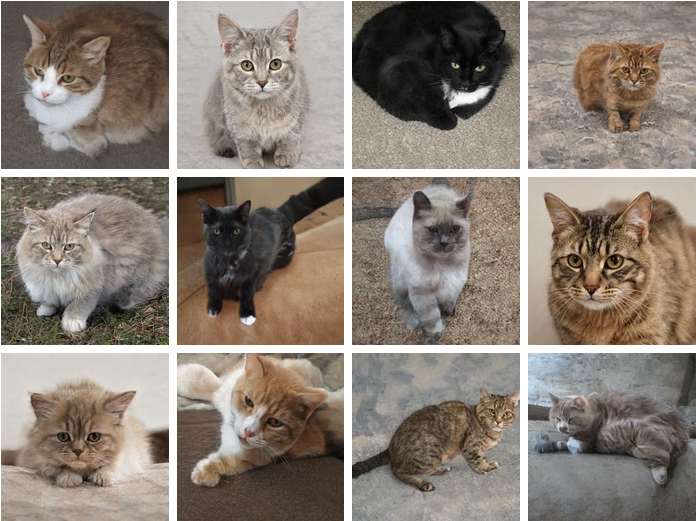
\includegraphics[width=\textwidth]{TCDNE.png}
        \end{column}
    \end{columns}
\end{frame}

\begin{frame}
    \frametitle{But Why?: Upscaling}
    \begin{columns}
        \begin{column}{0.48\paperwidth}
            \begin{itemize}
                \item We can take lossy images and produce higher quality
                    images.
                \item We can also take smaller images and make them larger.
                \item Helpful in compression.
                \item Restoration of images (also inpainting)
                \item Make old images/videos look new/modern.
            \end{itemize}
        \end{column}
        \begin{column}{0.48\paperwidth}
            \includegraphics[width=\textwidth]{Upscaling.jpg}
        \end{column}
    \end{columns}
\end{frame}

\begin{frame}
    \frametitle{But Why?: Learn Latent Variables}
    \begin{columns}
        \begin{column}{0.48\paperwidth}
            \begin{itemize}
                \item We can learn the different latent variables in a dataset.
                \item For example we can learn how to make someone old!
                \item We could also use this as a form of compression
                    (autoencoders)
                \item We can add/modify features of someone (add a mostache).
            \end{itemize}
        \end{column}
        \begin{column}{0.48\paperwidth}
            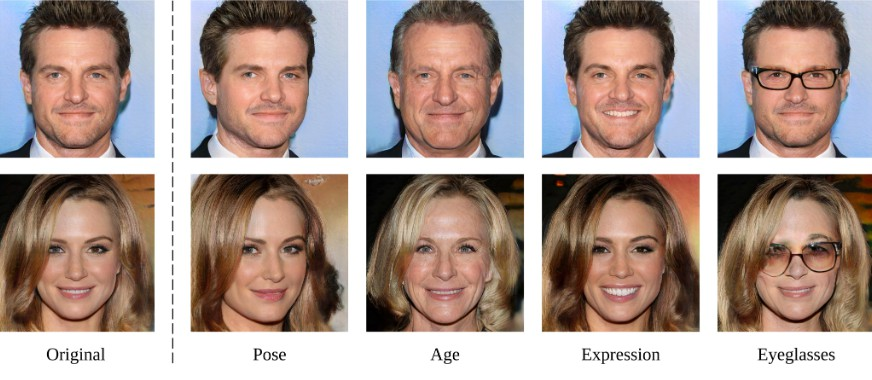
\includegraphics[width=\textwidth]{latent.jpg}
        \end{column}
    \end{columns}
\end{frame}

\begin{frame}
    \frametitle{But Why?: Uncovering Bias}
    \begin{columns}
        \begin{column}{0.48\paperwidth}
            \begin{itemize}
                \item<1-> Suppose we have a dataset of faces.
                \item<2-> Might have some distribution, let's say...
                \item<3-> Most of the faces fit in the main part of the
                    distribution.
                \item<4-> We have outliers in the dataset.
                \item<5-> We can now adjust our dataset (gather new data )or
                    potentially generate new images for a classifier if we can't
                    fix the distribution (might not be logistically possible).
            \end{itemize}
        \end{column}
        \begin{column}{0.48\paperwidth}
            \includegraphics<1>[width=\textwidth]{Faces.png}
            \includegraphics<2>[width=\textwidth]{Faces_Distribution.png}
            \includegraphics<3>[width=\textwidth]{Faces_MainDistrib.png}
            \includegraphics<4->[width=\textwidth]{Faces_Tail.png}
        \end{column}
    \end{columns}
\end{frame}


\begin{frame}
    \frametitle{Taxonomy of Generators}
    \includegraphics[width=\textwidth]{taxonomy.png}
    \null\hfill \tiny{source: ian goodfellow}
\end{frame}

\begin{frame}
    \frametitle{Taxonomy of Generators: Implicit Density}
    \begin{columns}
        \begin{column}{0.48\paperwidth}
            \begin{itemize}
                \item We want to learn a stochastic procedure to generate data. 
                \item We learn liklihood-free.
            \end{itemize}
        \end{column}
        \begin{column}{0.48\paperwidth}
            \includegraphics[width=\textwidth]{taxonomy_Implicit.png}
            \null\hfill \tiny{source: ian goodfellow}
        \end{column}
    \end{columns}
\end{frame}

\begin{frame}
    \frametitle{This X Does Not Exist}
    \vspace{-1em}
    \begin{figure}
        \begin{subfigure}{0.25\textwidth}
            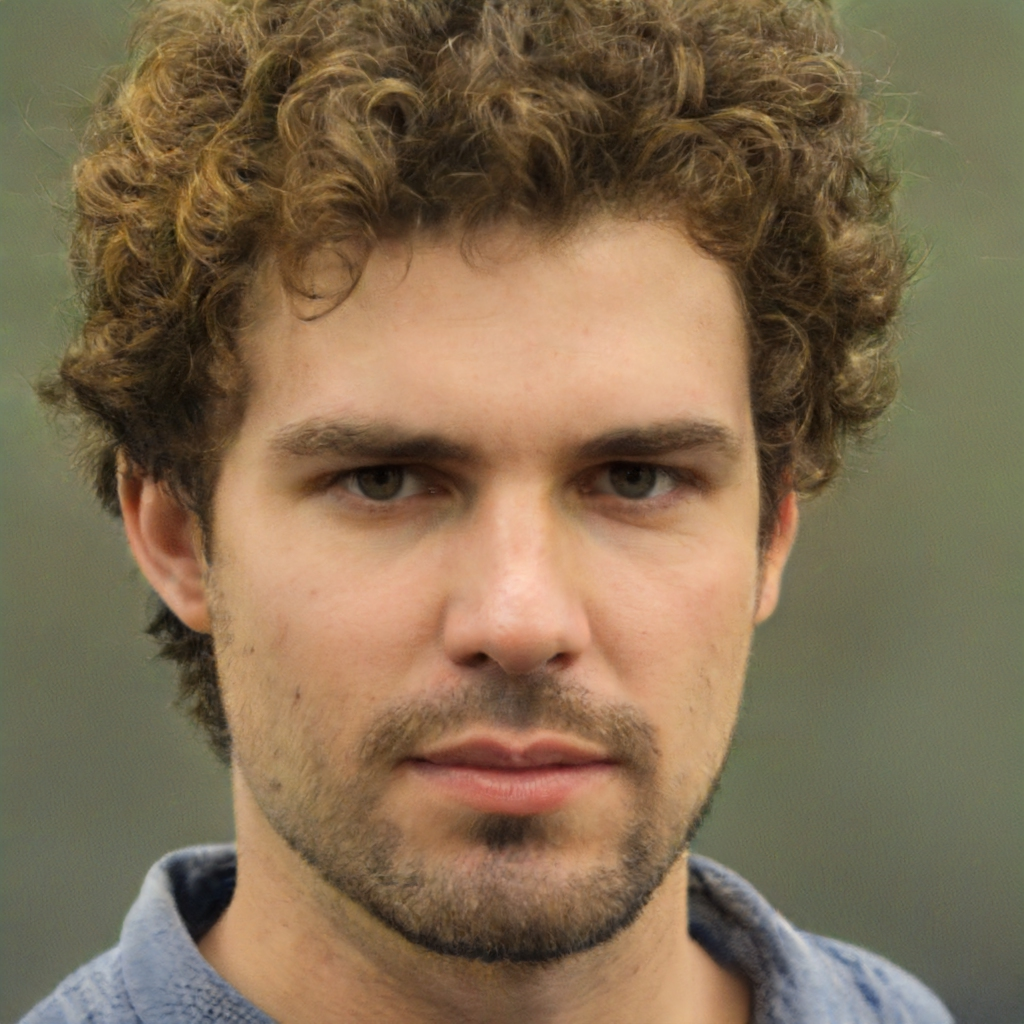
\includegraphics[width=\textwidth]{tpdne.jpg}
            \caption{This Person Does Not Exist (StyleGAN2)}
        \end{subfigure}
        \begin{subfigure}{0.25\textwidth}
            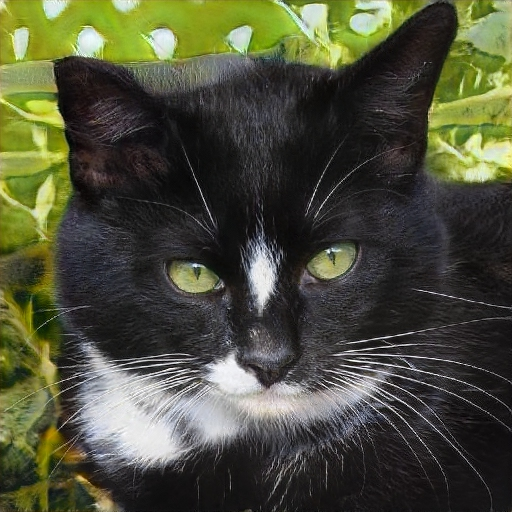
\includegraphics[width=\textwidth]{tcdne.jpg}
            \caption{This Cat Does Not Exist (StyleGAN)}
        \end{subfigure}
        \begin{subfigure}{0.5\textwidth}
            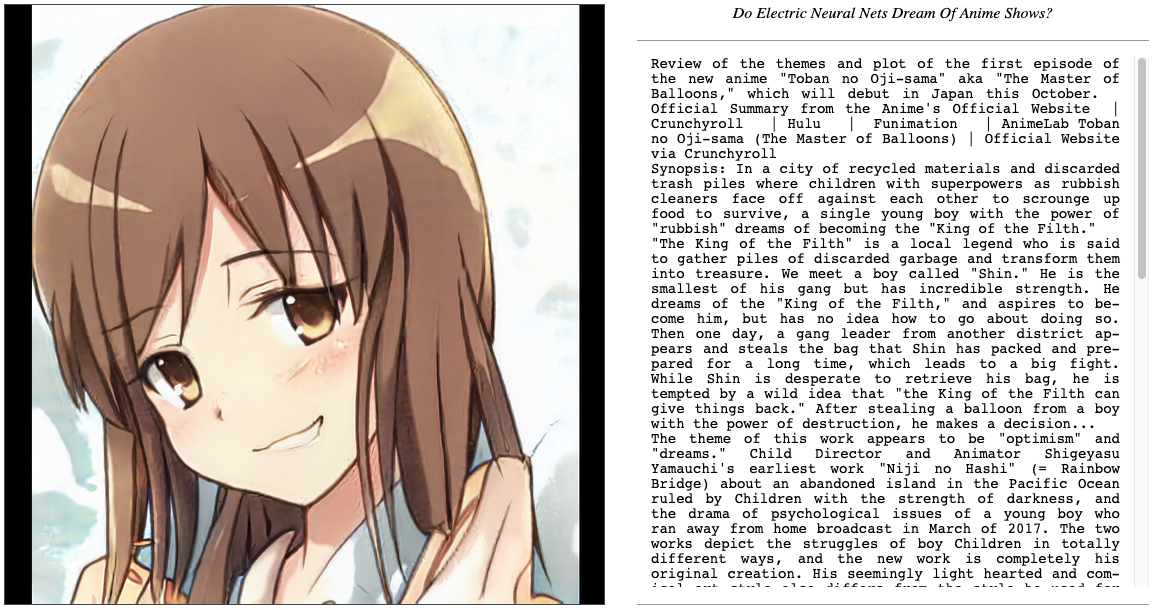
\includegraphics[width=\textwidth]{twdne.png}
            \caption{This Anime Does Not Exist (StyleGAN2 + GPT-3)}
        \end{subfigure}
    \end{figure}
\end{frame}

\begin{frame}
    \frametitle{Generative Adversarial Networks}
    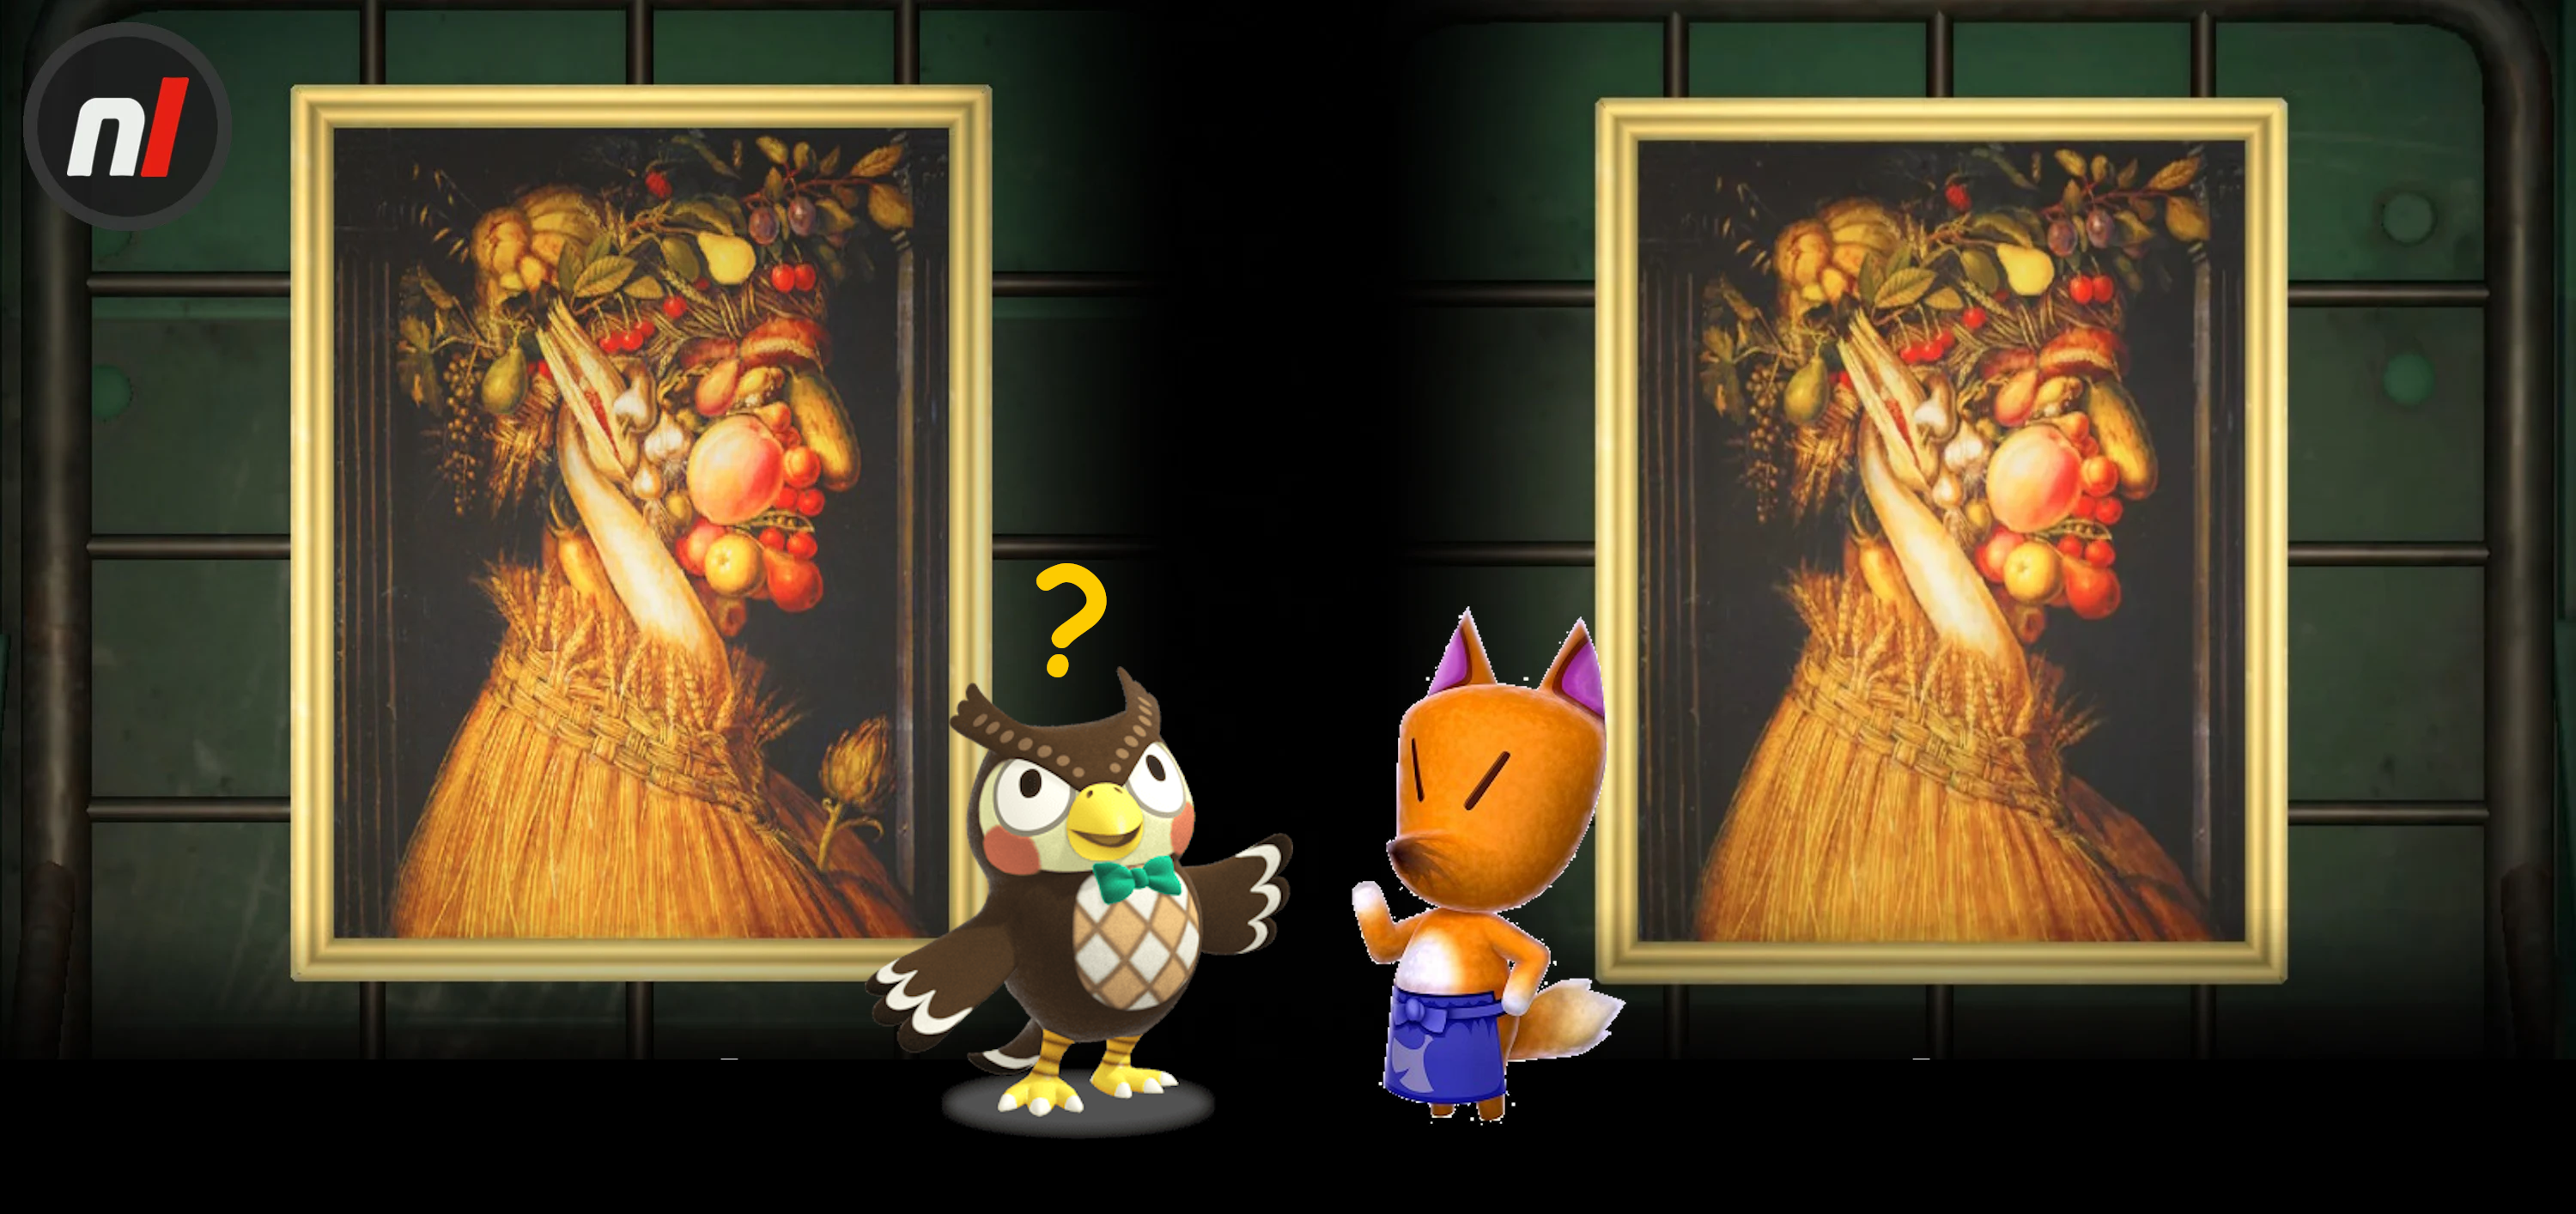
\includegraphics[width=\textwidth]{AC-GAN.png}
\end{frame}

\begin{frame}
    \frametitle{Generative Adversarial Networks}
    \center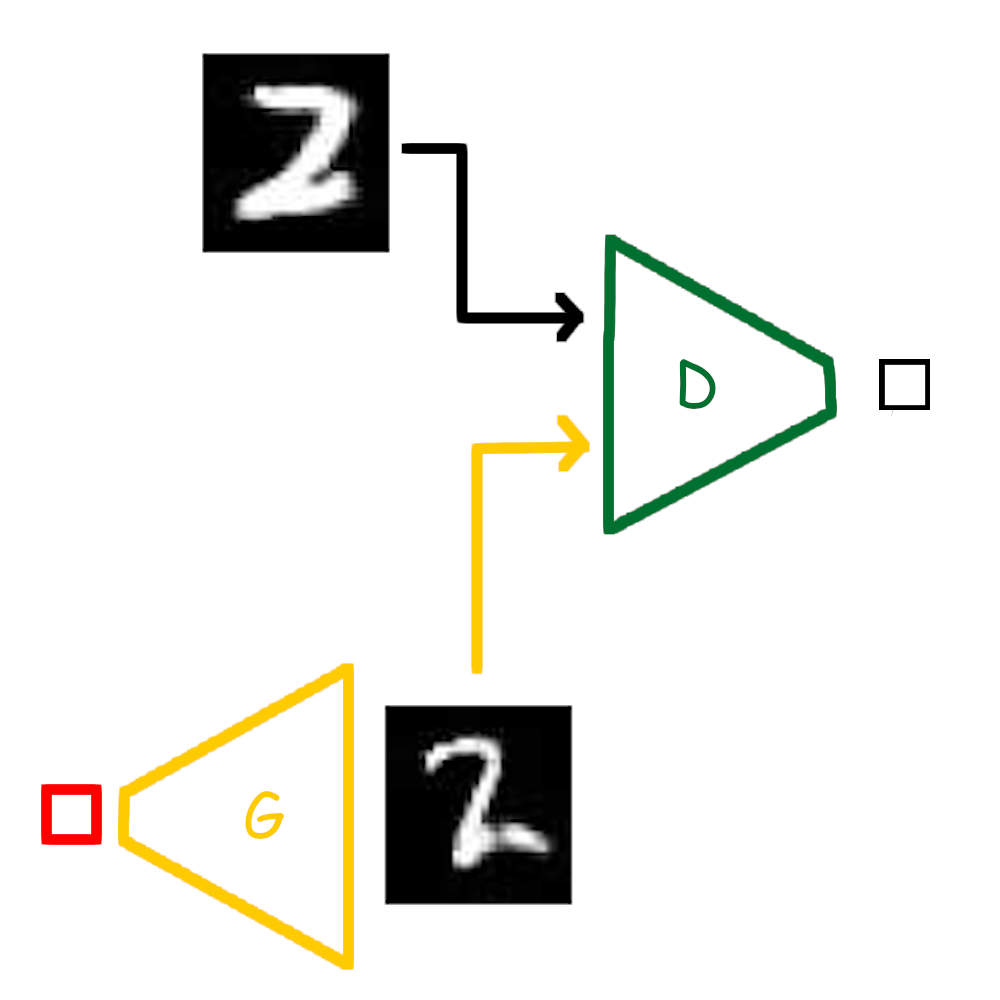
\includegraphics[height=0.75\textheight]{GAN.png}
\end{frame}

\begin{frame}
    \frametitle{Generative Adversarial Networks}
    \center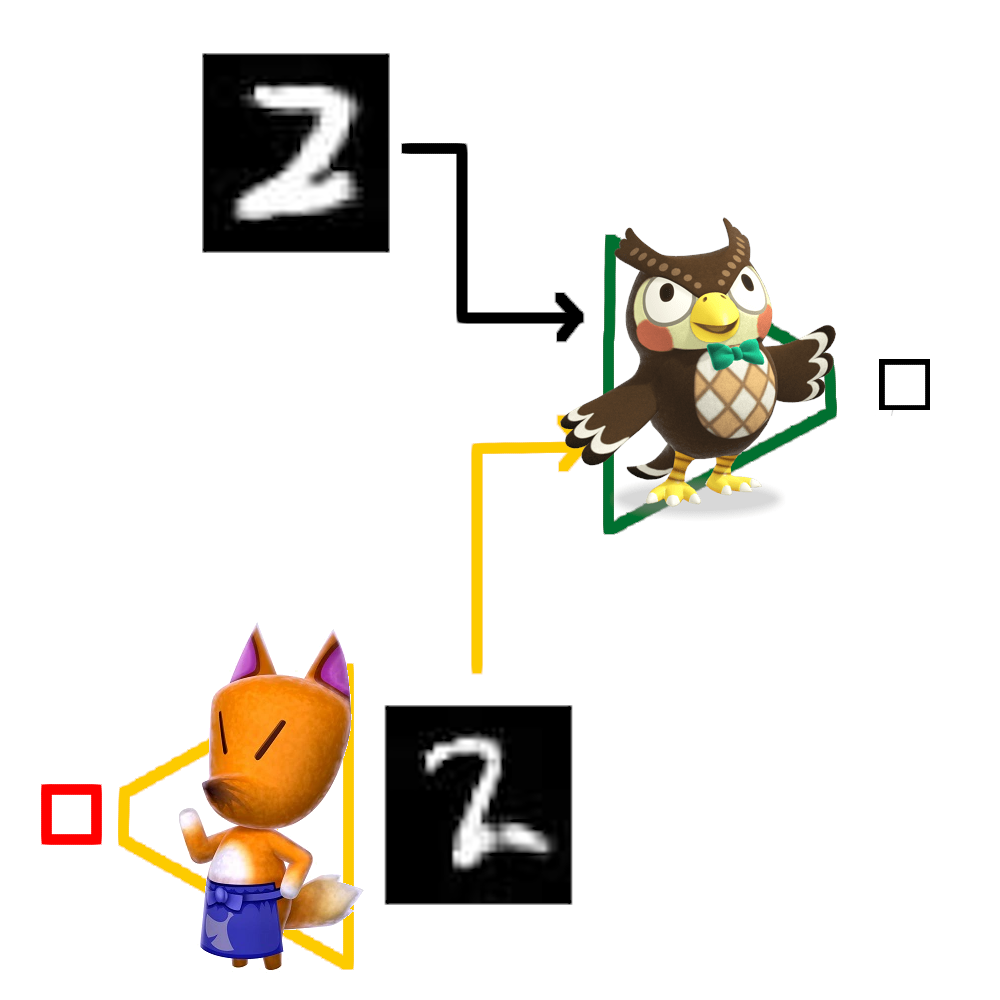
\includegraphics[height=0.75\textheight]{GAN-as-AC.png}
\end{frame}

\begin{frame}
    \frametitle{Generative Adversarial Networks}
    \begin{itemize}
        \item Send noise into Generator.
        \item Send generated image and real images into Discriminator.
        \item Play mini-max game teaching the Generator to fool the
            Discriminator.
        \item When fake image can adaquately fool (a well trained) discriminator
            we produce quality images. 
        \item<2-> In practice we train D, then G then repeat. 
    \end{itemize}
\end{frame}

\begin{frame}
    \frametitle{But Why Is This Implicit?}
    \begin{itemize}
        \item We didn't learn a density function.
        \item We just focus on generating samples.
        \item Don't have an (easy) smooth transition between latent variables.
        \item Likelihood is not tractable.
        \item "We're training them to memorize, not generalize" - Ian Goodfellow
    \end{itemize}
\end{frame}

\begin{frame}
    \frametitle{Latent Space}
    \includegraphics<1>[height=0.75\textheight]{oregonTopo.jpg}
    \includegraphics<2>[height=0.75\textheight]{oregonTopo1.jpg}
    \includegraphics<3>[height=0.75\textheight]{oregonTopo2.jpg}
    \includegraphics<4>[height=0.75\textheight]{oregonTopo3.jpg}
    \includegraphics<5>[height=0.75\textheight]{oregonTopo4.jpg}
\end{frame}

\begin{frame}
    \frametitle{Latent Space}
    \vspace{-1.25em}
    \center\footnotesize{TSNE visualization of vanilla GAN latent space. }
    \center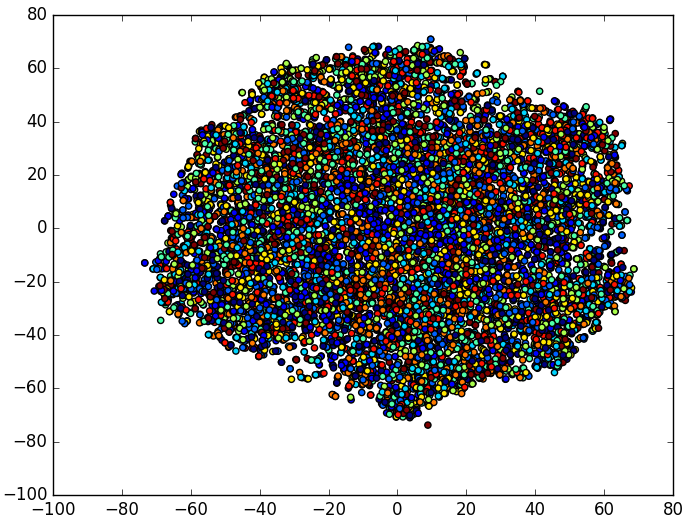
\includegraphics[height=0.70\textheight]{GANLatent.png}
    \\
    \tiny{Image from ClusterGAN paper which works on resolving this
    issue}
\end{frame}

\begin{frame}
    \frametitle{So Why Use GANs?}
    \begin{itemize}
        \item Because they are quick.
        \item They produce high quality images.
        \item Can still do many tasks.
        \item They're well researched.
    \end{itemize}
\end{frame}

\begin{frame}
    \frametitle{StyleGAN2}
    Let's look at a modern GAN and how it works.
\end{frame}

\begin{frame}
    \frametitle{Problems With StyleGAN}
    \begin{itemize}
        \item GANs typically have ``blobs'' that are mysteriously produced.
        \item Often get ``GAN Monsters'' where parts of images get wildly
            distorted.
        \item Certain characteristics are too common. Eyes forward, smile
            alignment. 
    \end{itemize}
\end{frame}

\begin{frame}
    \frametitle{Blobs and More Blobs}
    \center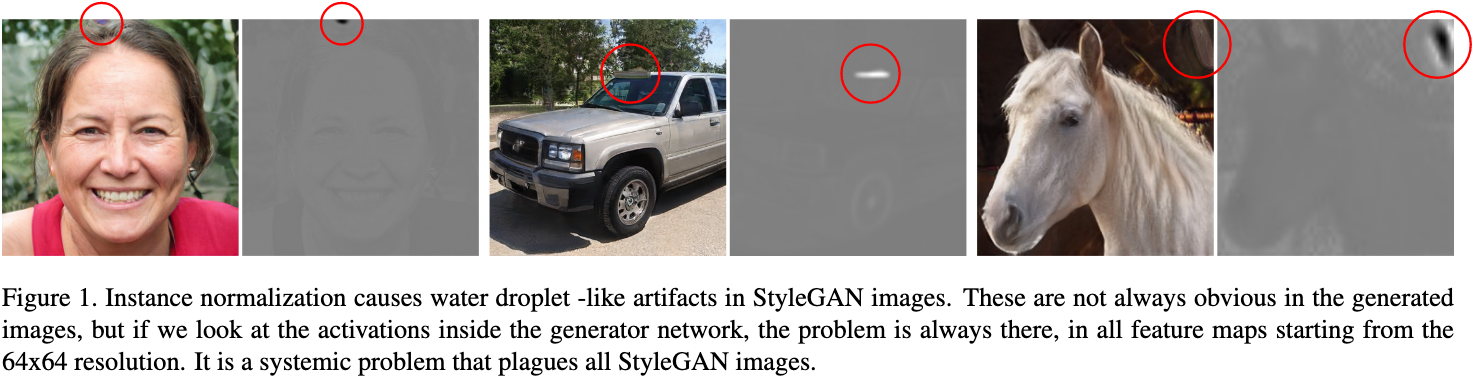
\includegraphics[width=\textwidth]{StyleGAN2_blobs.png}
\end{frame}

\begin{frame}
    \frametitle{Monsters}
    \center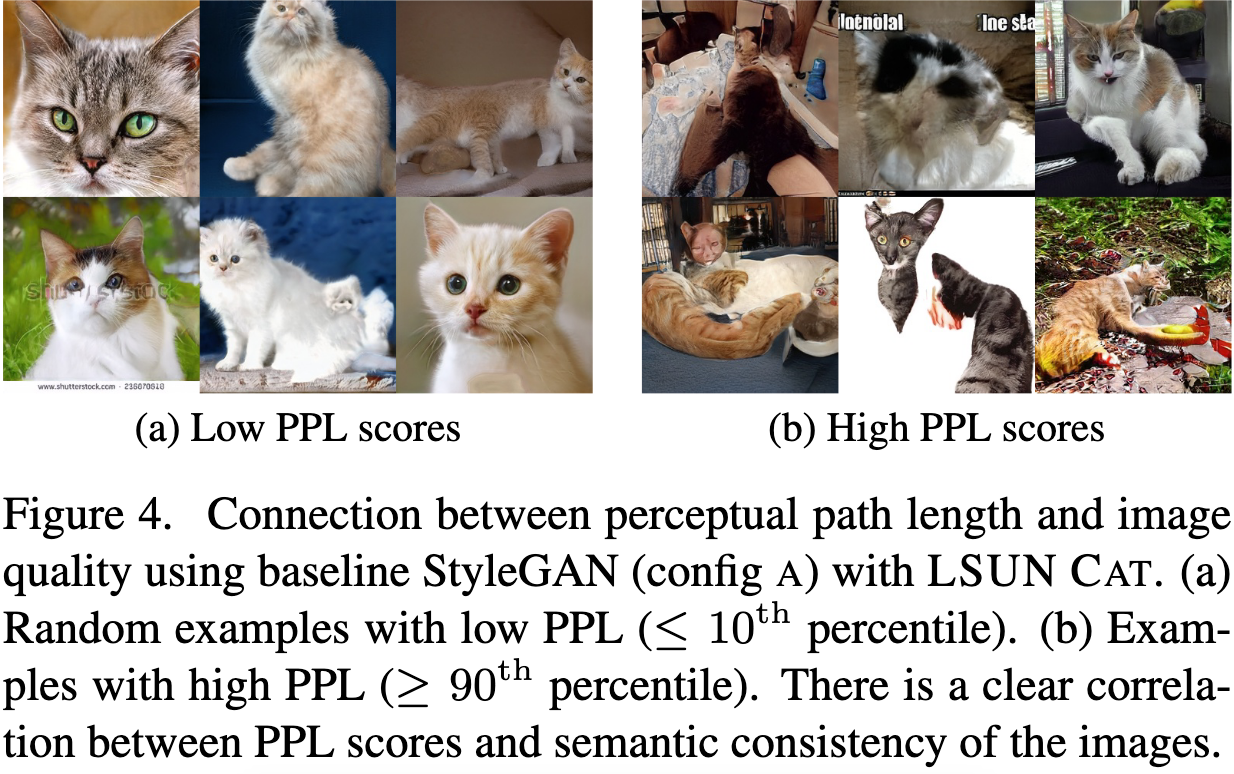
\includegraphics[width=\textwidth]{StyleGAN2_monsters.png}
\end{frame}

\begin{frame}
    \frametitle{Phase Characteristics}
    \center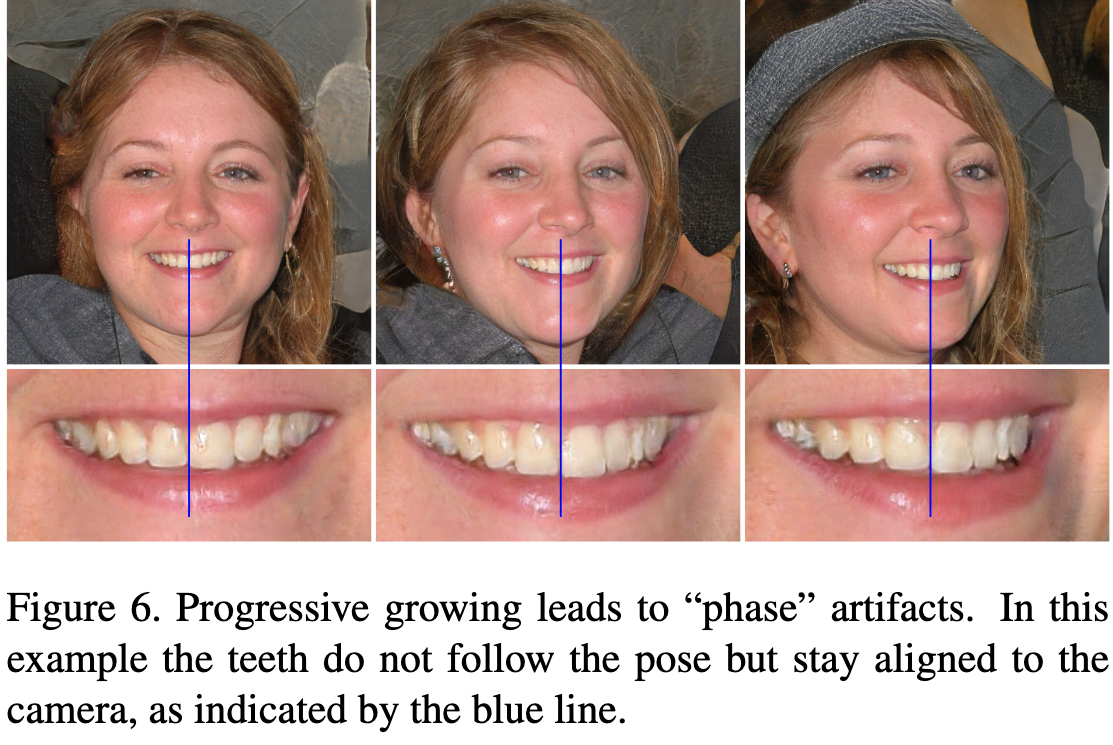
\includegraphics[width=\textwidth]{StyleGAN2_phase.png}
\end{frame}

\begin{frame}
    \frametitle{StyleGAN (OG)}
    \center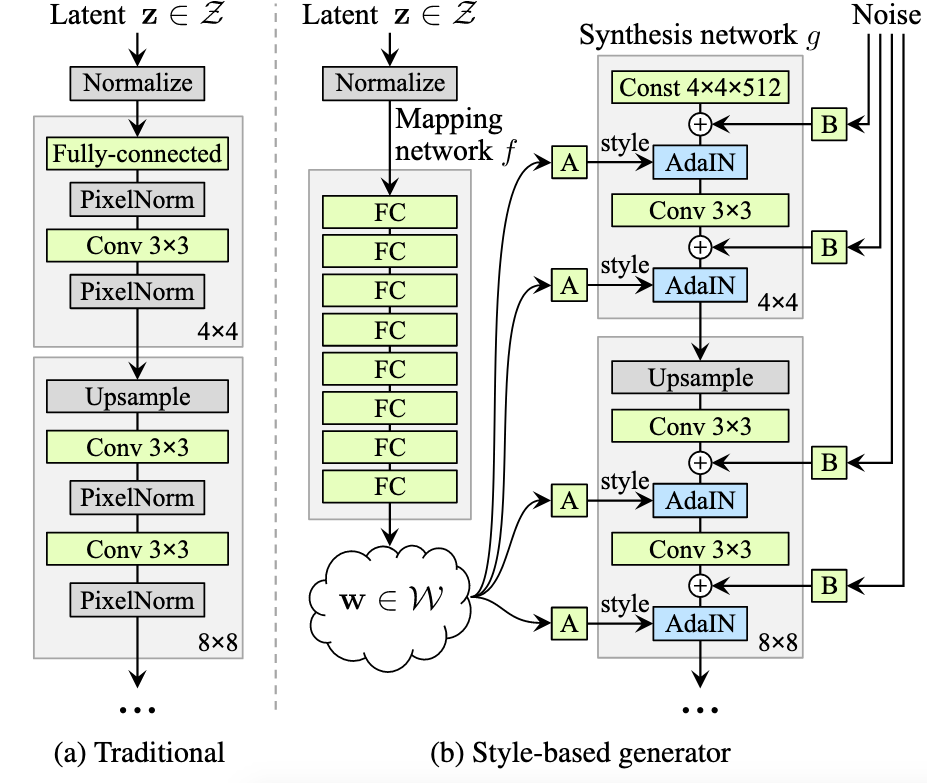
\includegraphics[width=\textwidth]{StyleGAN.png}
\end{frame}

\begin{frame}
    \frametitle{StyleGAN (OG)}
    \begin{columns}
        \begin{column}{0.48\paperwidth}
            \begin{itemize}
                \item Uses upscaling convolutions, doubling.
                \item Learns a ``style space'' ($w$)
                \item Introduces Adaptive Instance Normalization (AdaIN)\\
                    AdaIN$(x_i,y) = y_{s,i}\frac{x_i - \mu(x_i)}{\sigma(x_i)} +
                    y_{b,i}$
            \end{itemize}
        \end{column}
        \begin{column}{0.48\paperwidth}
            \center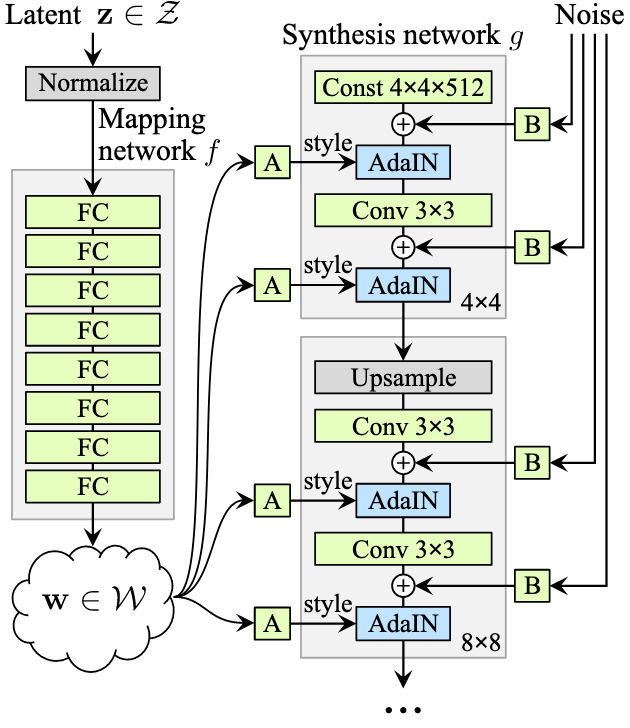
\includegraphics[width=\textwidth]{StyleGAN_only.png}
        \end{column}
    \end{columns}
\end{frame}

\begin{frame}
    \frametitle{StyleGAN vs StyleGAN 2}
    \center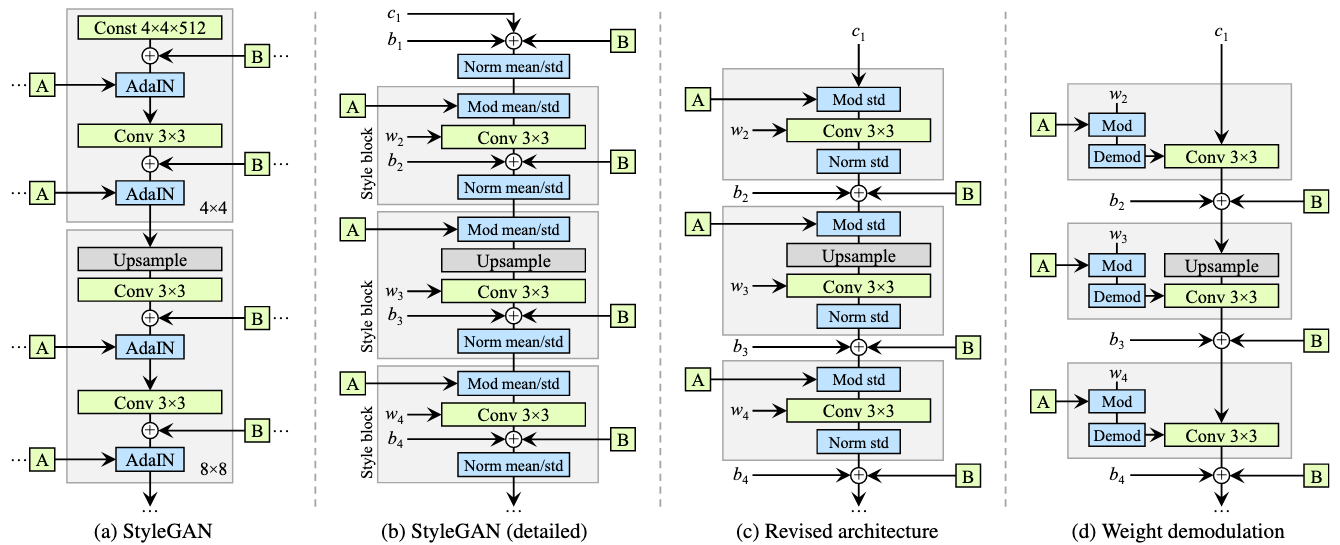
\includegraphics[width=\textwidth]{StyleGAN1And2.png}
\end{frame}

\begin{frame}
    \frametitle{StyleGAN2: What Changed}
    \begin{itemize}
        \item Removed AdaIN. Removing this removes the droplet/blobs.
        \item Lazy Regularization: Split loss and regularization terms and
            regularize every 16 minibatches.
        \item Noticed low Perceptual Path Length (PPL) results had better images
            so introduced a new regularizer to account for this.
        \item Use skip generator and residual discriminator instead of
            progressive growing.
        \item Increase network size (helps get from 512x512 to 1024x1024).
    \end{itemize}
\end{frame}

\begin{frame}
    \frametitle{StyleGAN2 Results}
    \center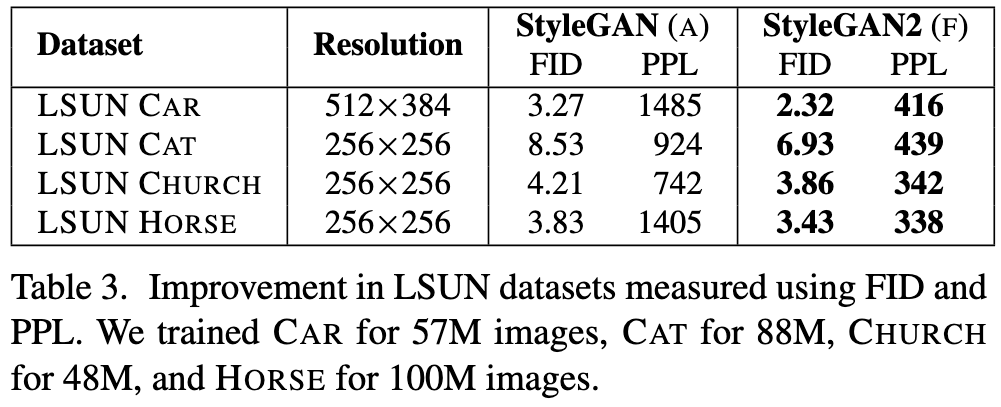
\includegraphics[width=\textwidth]{StyleGAN2_results.png}
\end{frame}

\begin{frame}
    \frametitle{StyleGAN2 Results}
    \center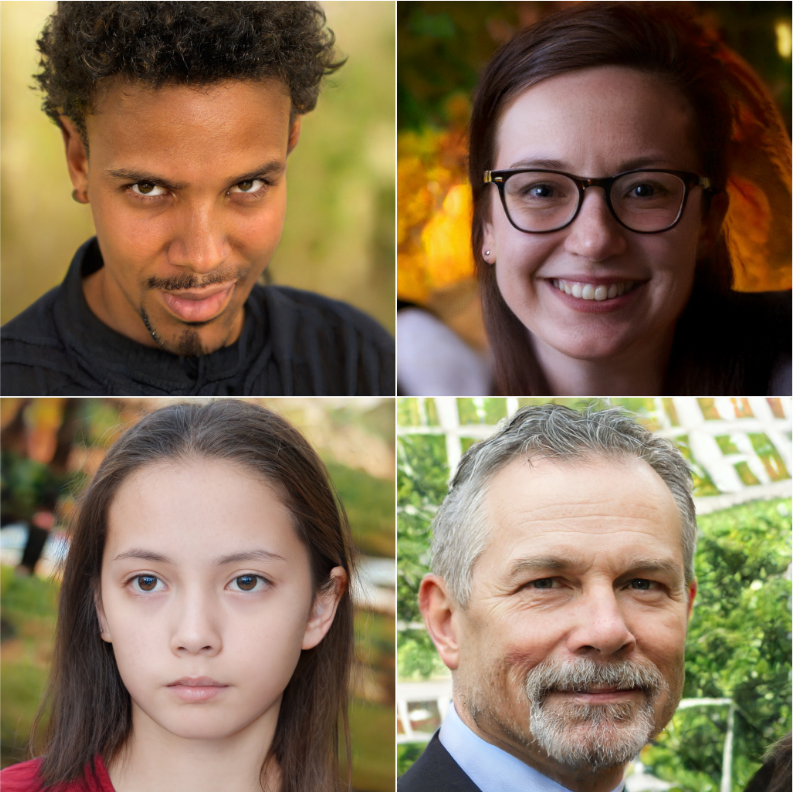
\includegraphics[width=\textwidth]{StyleGAN2_hand.png}
\end{frame}

\begin{frame}
    \frametitle{Taxonomy of Generators: Explicit Density}
    \begin{columns}
        \begin{column}{0.48\paperwidth}
            \begin{itemize}
                \item We want to learn a distribution of
                    data. 
                \item We assume some prior about the distribution of the data. 
                \item We learn the log-liklihood of the function $\log
                    p_\theta(x)$
            \end{itemize}
        \end{column}
        \begin{column}{0.48\paperwidth}
            \includegraphics[width=\textwidth]{taxonomy_Explicit.png}
            \null\hfill \tiny{source: ian goodfellow}
        \end{column}
    \end{columns}
\end{frame}

\begin{frame}
    \frametitle{AutoEncoders}
    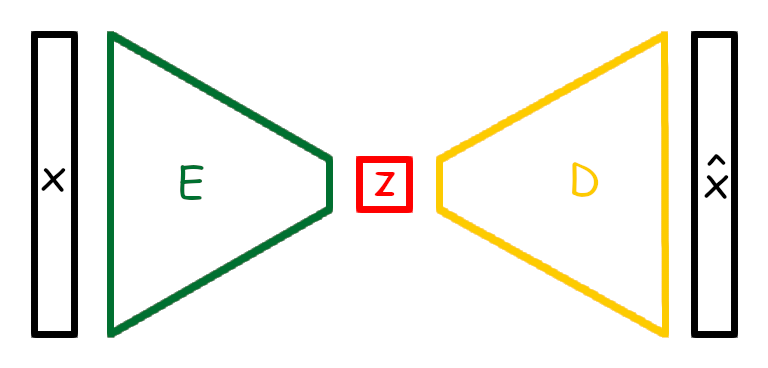
\includegraphics[width=\textwidth]{AutoEncoder.png}
\end{frame}


\begin{frame}
    \frametitle{AutoEncoders}
    \begin{columns}
        \begin{column}{0.48\paperwidth}
            \begin{itemize}
                \item Want to learn latent variable $z$ from $x$. $\mathbb{R}^n
                    \mapsto \mathbb{R}^m$ where $m<n$
                \item Compressed representation of the data.
                \item Since we don't have training data for z, we construct a
                    decoder to do unsupervised learning.
            \end{itemize}
        \end{column}
        \begin{column}{0.48\paperwidth}
            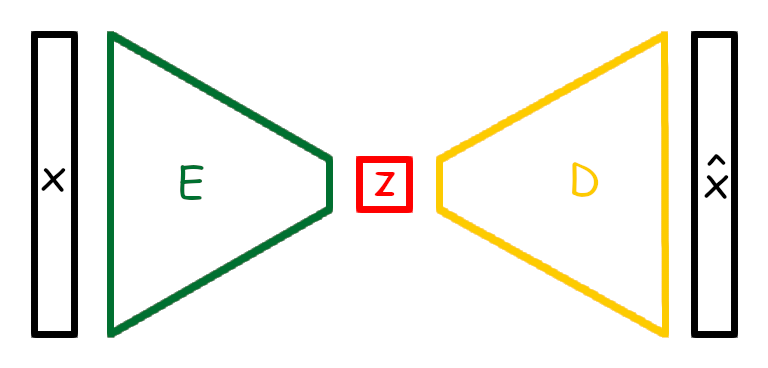
\includegraphics[width=\textwidth]{AutoEncoder.png}
        \end{column}
    \end{columns}
\end{frame}

\begin{frame}
    \frametitle{AutoEncoders}
    \begin{columns}
        \begin{column}{0.48\paperwidth}
            \begin{itemize}
                \item<1-> Want to take $x$ and produce $\hat{x}$
                \item<2-> Sample $x$ from dataset and encode to latent space
                    $z$.
                \item<3-> Decode to sample from $z$ and generate $\hat{x}$
                \item<4-> Regularize $||x-\hat{x}||^2$
                \item<5-> Gives us a unsupervised training.
            \end{itemize}
        \end{column}
        \begin{column}{0.48\paperwidth}
            \includegraphics<1>[width=\textwidth]{AutoEncoder_blank.png}
            \includegraphics<2>[width=\textwidth]{AutoEncoder_In.png}
            \includegraphics<3>[width=\textwidth]{AutoEncoder_Out.png}
            \includegraphics<4->[width=\textwidth]{AutoEncoder_Reg.png}
        \end{column}
    \end{columns}
\end{frame}

\begin{frame}
    \frametitle{Pick Our Latent Space Size Carefully}
    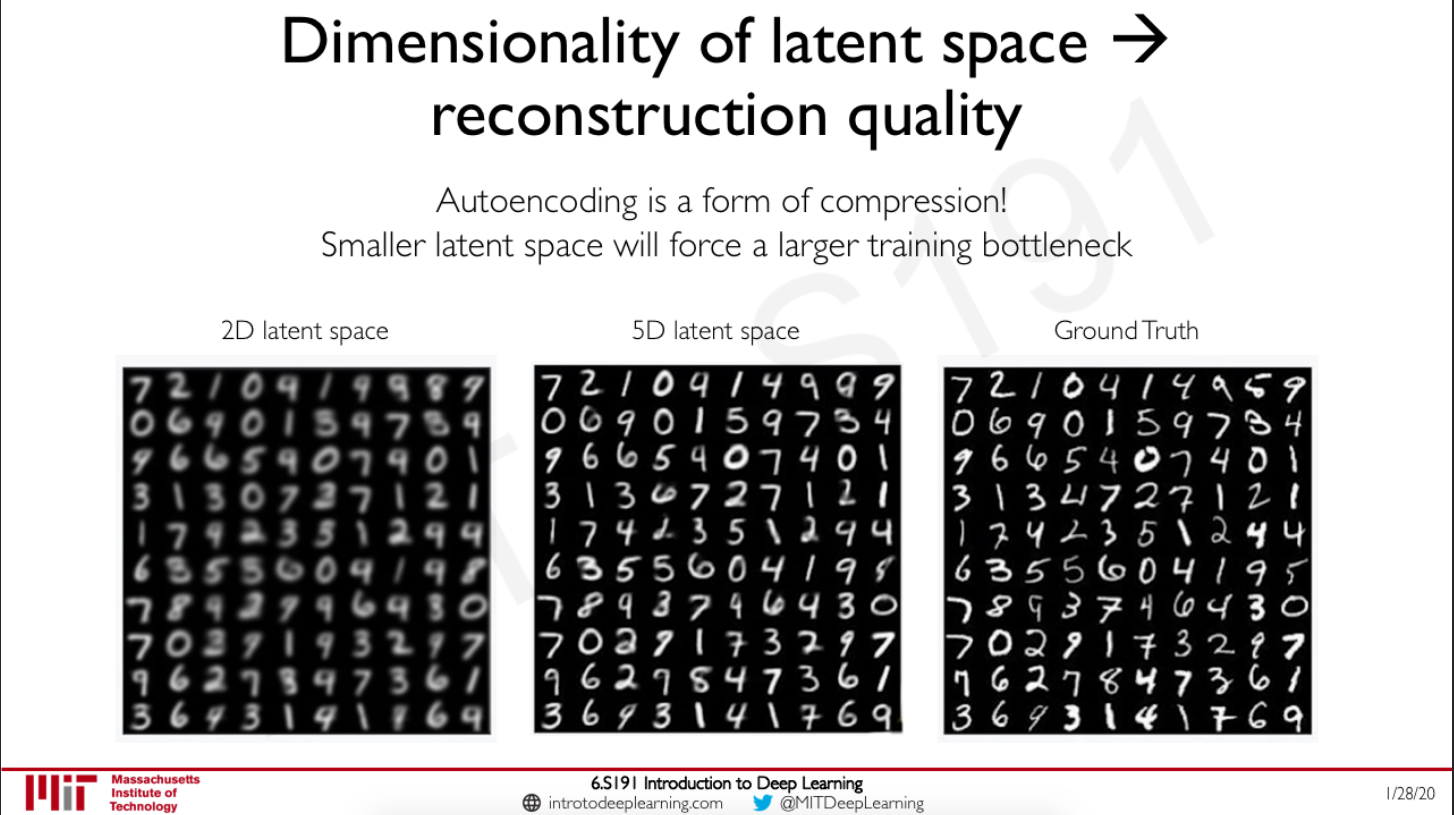
\includegraphics[width=\textwidth]{AE-MNIST.png}
\end{frame}

\begin{frame}
    \frametitle{The BIG Problem!}
    \center We can't generate new and unique samples!
\end{frame}

\begin{frame}
    \frametitle{Taxonomy of Generators}
    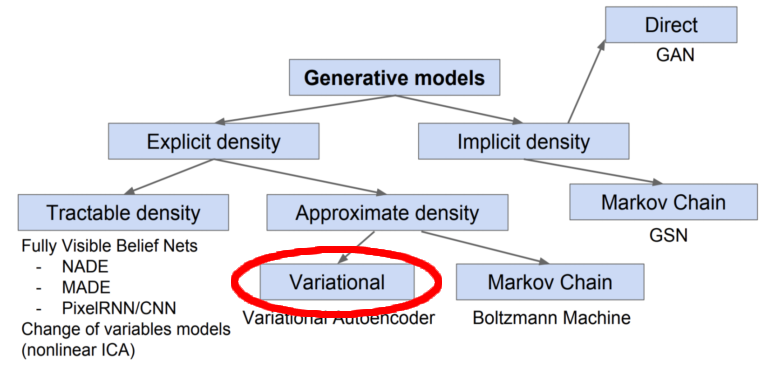
\includegraphics[width=\textwidth]{Taxonomy_VAE.png}
    \null\hfill \tiny{source: ian goodfellow}
\end{frame}

\begin{frame}
    \frametitle{Variational Autoencoder (VAE)}
    \begin{itemize}
        \item We need a way to generate \textbf{new} samples that aren't seen in
            the dataset.
        \item Need to add some variance and noise (make non-determanistic).
        \item Still have to be able to do back propagation.
    \end{itemize}
\end{frame}

\begin{frame}
    \frametitle{VAE: Breaking Down the Problem}
    \begin{itemize}
        \item<1-> Suppose there is some hidden (latent) variable $z$ that produces
            observation $x$, $p(z|x)$. \textbf{We want to learn this.}
        \item<2-> $p(z|x) = \frac{p(x|z)p(z)}{p(x)}$
        \item<3-> $p(x) = \int p(x|z)p(z)dz$ (intractable!)
        \item<4-> We can approximate $p(z|x)$ with another distribution $q(z|x)$
            that is tractable.
        \item<5-> We'll then need to measure the difference between $p$ and $q$.
    \end{itemize}
\end{frame}

\begin{frame}
    \frametitle{Variational Autoencoder (VAE)}
    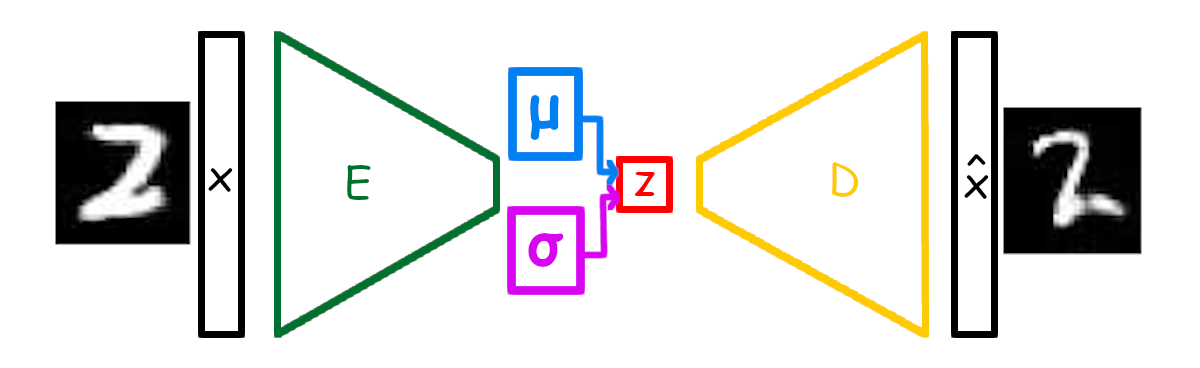
\includegraphics[width=\textwidth]{VAE.png}
\end{frame}

\begin{frame}
    \frametitle{Variational Autoencoder (VAE)}
    \begin{columns}
        \begin{column}{0.60\paperwidth}
            \begin{itemize}
                \item<1-> Encoder computes $p_\phi(z|x)$ \\(reconstruction loss, like
                    autoencoder)
                \item<2-> Decoder computes $q_\theta(x|z)$ \\(regularization term)
                \item<3-> $L(\phi,\theta,x) = ||x - \hat{x}||^2 + KL(p_\phi(z|x)
                    || p(x))$
            \end{itemize}
        \end{column}
        \begin{column}{0.40\paperwidth}
            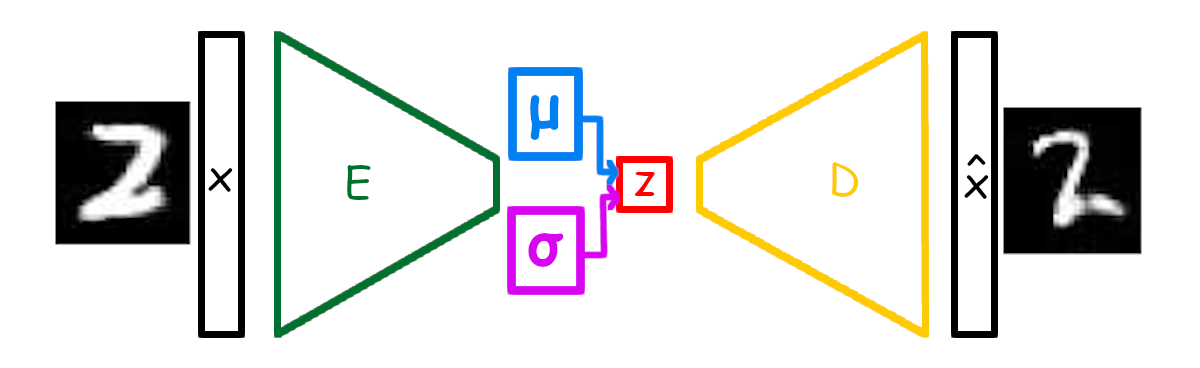
\includegraphics[width=\textwidth]{VAE.png}
        \end{column}
    \end{columns}
\end{frame}

\begin{frame}
    \frametitle{(VAE) Regularization Term}
    \begin{columns}
        \begin{column}{0.60\paperwidth}
            \begin{itemize}
                \item $L(\phi,\theta,x) = ||x - \hat{x}||^2 + KL(p_\phi(z|x)
                    || p(x))$
                \item We are using the KL-Divergence between the
                    \textit{inferred latent distribution} ($p_\phi(z|x)$) and
                    the \textit{fixed prior on latent distribution} ($p(z)$).
                \item What prior? Why not Gaussian? $p(z) =
                    \mathcal{N}(\mu=0, \sigma^2=1)$
                \item Encourages encoding to distribute evenly around latent
                    space and penalizes when memorizing.
                \item $KL(p_\phi(z|x) || p(z)) = -\frac12\sum(\sigma_j +
                    \mu_j^2 - 1 -\log{\sigma_j})$
            \end{itemize}
        \end{column}
        \begin{column}{0.40\paperwidth}
            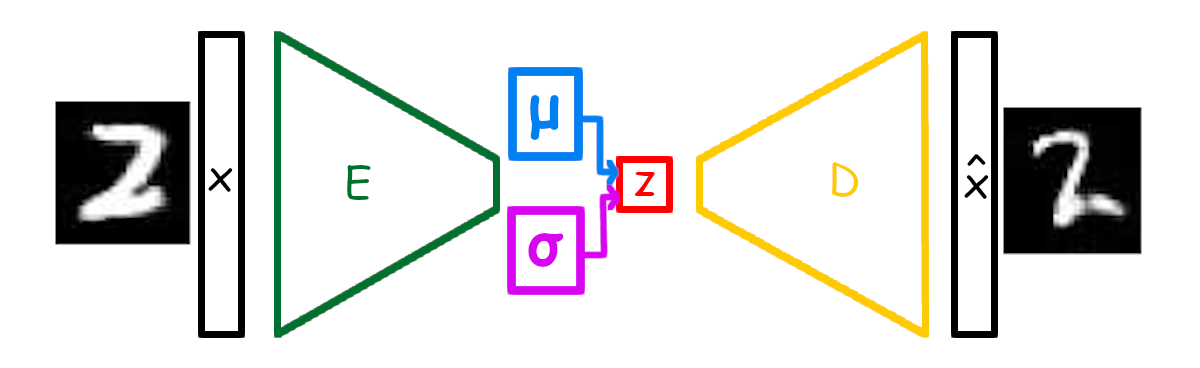
\includegraphics[width=\textwidth]{VAE.png}
        \end{column}
    \end{columns}
\end{frame}

\begin{frame}
    \frametitle{(VAE) Reparameterization}
    \begin{columns}
        \begin{column}{0.60\paperwidth}
            \begin{itemize}
                \item<1-> Ops! We can't backprop through this! $z$ is a
                    stochastic node.
                \item<2-> We can reparameratize.
                \item<3-> $z = \mu + \sigma \odot \varepsilon$
                \item<3-> We let $\mu$ and $\sigma$ be fixed vectors and
                    $\varepsilon \sim \mathcal{N}(0,1)$
                \item<4-> Now we can backprop through $\phi$ and $x$. 
                \item<4-> Now we can adjust $\varepsilon$ and create new images
                    similar to the ones we learned from.
            \end{itemize}
        \end{column}
        \begin{column}{0.40\paperwidth}
            \centering\includegraphics<1-2>[width=0.5\textwidth]{VAE-beforeReParam.png}
            \centering\includegraphics<3->[width=0.7\textwidth]{VAE-ReParam.png}
        \end{column}
    \end{columns}
\end{frame}

\begin{frame}
    \frametitle{Approximate Density Estimation}
    \begin{itemize}
        \item We didn't actually learn $p(x)$ but rather $q(x)$.
        \item We approximated the density of $p(x)$ with a tractable
            distribution.
        \item KL Divergence is always $\geq 0$.
    \end{itemize}
\end{frame}

\begin{frame}
    \frametitle{Good and Bad of a VAE}
    \begin{itemize}
        \item They are very easy to train.
        \item Often not high quality images.
        \item You learn an approximate density function (have log-liklihood)
    \end{itemize}
\end{frame}

\begin{frame}
    \frametitle{Taxonomy of Generators}
    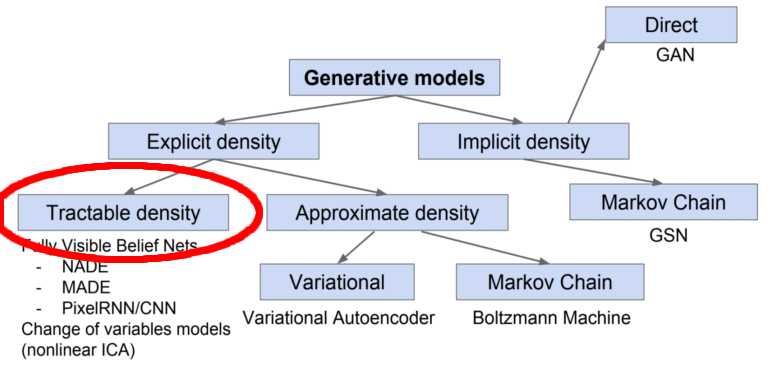
\includegraphics[width=\textwidth]{Taxonomy_Tractable.png}
    \null\hfill \tiny{source: ian goodfellow}
\end{frame}

\begin{frame}
    \frametitle{Density Estimation}
    \begin{itemize}
        \item We've come close to learning density, but not exactly. 
        \item Density is \textbf{very} difficult to learn.
        \item Having true density \textit{should} mean better ability to perform
            our downstream tasks (generation, density estimation, latent
            variable inference, etc)
    \end{itemize}
\end{frame}

\begin{frame}
    \frametitle{Change Of Variables}
    \begin{columns}
        \begin{column}{0.49\paperwidth}
            \begin{itemize}
                \item What if we just map to a different space?
                \item We'll convert one probability distribution to another
                    tractable distribution (such as a Gaussian)
            \end{itemize}
        \end{column}
        \begin{column}{0.49\paperwidth}
            \center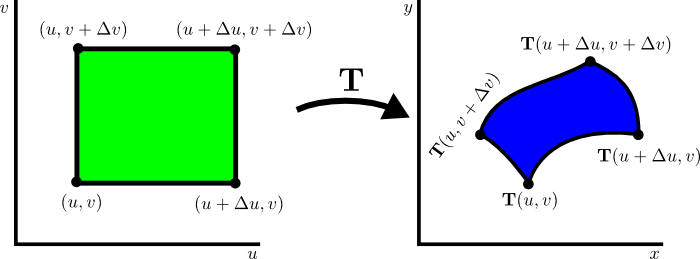
\includegraphics[width=\textwidth]{cov.png}
        \end{column}
    \end{columns}
\end{frame}

\begin{frame}
    \frametitle{Bijection (One-to-One and On-To)}
    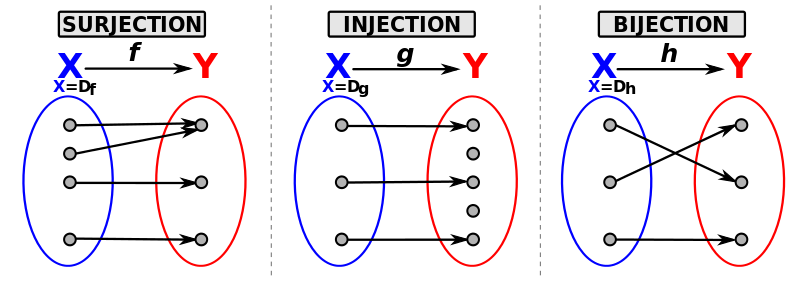
\includegraphics[width=1.\textwidth]{bijective.png}
\end{frame}

\begin{frame}
    \frametitle{Change Of Variables}
    \begin{itemize}
        \item<1-> $\int p(x)dx = \int q(z)dz = 1$ (Definition of PDF)
        \item<2-> $p(x) = q(z) \left | \frac{dz}{dx} \right |$
        \item<3-> $= q(f^{-1}(x))\left | \frac{df^{-1}(x)}{dx}\right |$
        \item<4-> $p(x) = q(f^{-1}(x))\left | det\frac{df^{-1}(x)}{dx} \right |$
            (using the Jacobian determinant)
    \end{itemize}
\end{frame}

\begin{frame}
    \frametitle{Normalizing Flow}
    \center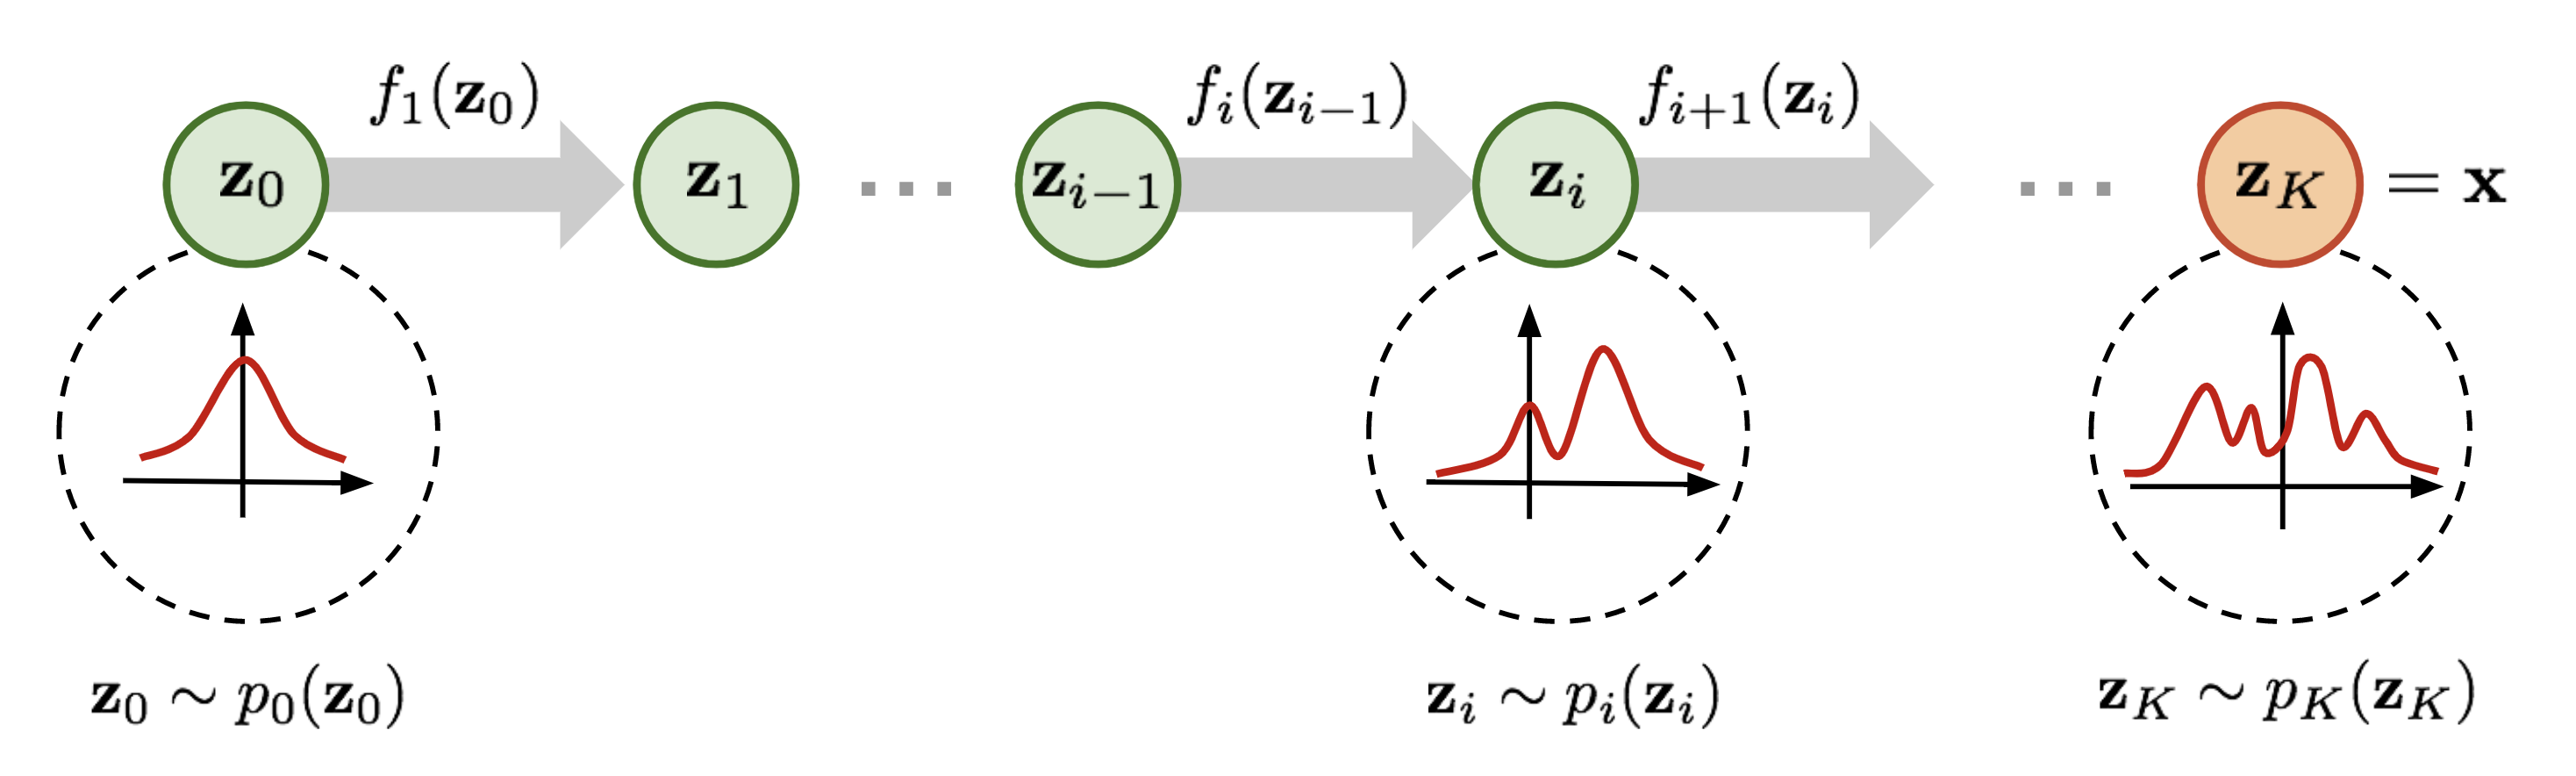
\includegraphics[width=\textwidth]{normalizing-flow.png}
    \tiny{Source: lilianweng.github.io}
\end{frame}

\begin{frame}
    \frametitle{Normalizing Flow}
    \begin{itemize}
        \item We need our function $f(x)$ to be easily invertible
        \item The Jacobian determinant needs to be \textit{easy} to compute.
        \item BUT we get the exact log-likelihood of $p(x)$ (tractable) and we
            can train our model on the NLL \\$\mathcal{L}(D) = -\frac{1}{|D|}
            \sum\limits_{x\in D} log{p(x)}$
    \end{itemize}
\end{frame}

\begin{frame}
    \frametitle{NICE: Non-linear Independent Components Estimation}
    \begin{itemize}
        \item<1-> Key Idea: What if split the the transformation into two
            blocks? $x \mapsto (x_0, x_1)$
        \item<2-> Use an easy to invert equation.\\
            \begin{tabular}{|l|l|}
                \hline
                $f(x)$ & $f^{-1}(y)$\\
                \hline
                $y_0 = x_0$ & $x_0 = y_0$\\
                $y_1 = x_1 + m(x_0)$ & $x_1 = y_1 - m(y_0)$
                \\\hline
            \end{tabular}
        \item<3->Jacobian is trivial and triangular.
        \item<4->2nd Key Idea: Permute $x$ split: $x_0 \mapsto (x_{0,0}, x_{0,1}), x_1
            \mapsto (x_{1,1}, x_{1,0}), x_2 \mapsto...$
    \end{itemize}
\end{frame}

\begin{frame}
    \frametitle{Throwing It Together}
    \begin{itemize}
        \item Sample from a tractable distribution $z\sim f(x)$.
        \item Make $m(x)$ a neural net.
        \item Use at least 3 layers (permuting $x$).
        \item Add a scaling term at the last layer $e^s\odot f(x)$.
    \end{itemize}
    \center\includegraphics[width=0.6\textwidth]{permute.png}
\end{frame}

\begin{frame}
    \frametitle{NICE: Results}
    \center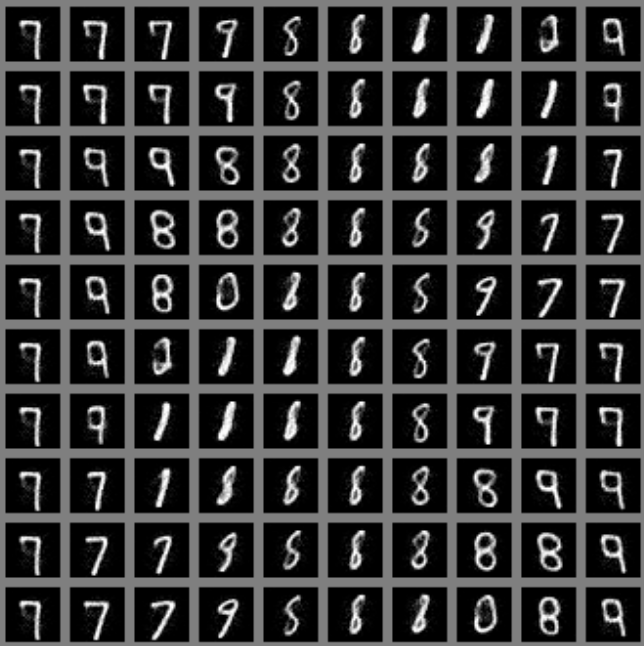
\includegraphics[width=0.65\textwidth]{NICEMNIST.png}
\end{frame}

\begin{frame}
    \frametitle{Why Is This Better/Worse?}
    \begin{itemize}
        \item We've learned a richer family of priors compared to VAE.
        \item More difficult to train because we need invertible functions.
        \item Able to perform complex/accurate downstream tasks because we've
            better approximated the distribution. (e.g. Inpainting, conceptual
            compression)
    \end{itemize}
\end{frame}

\begin{frame}
    \frametitle{GLOW}
    \begin{itemize}
        \item NICE (and RealNVP) do not produce sharp images.
        \item NICE could not compete with common GAN tasks like face generation.
        \item Need a new model to get sharp features and produce high quality
            images. 
    \end{itemize}
\end{frame}

\begin{frame}
    \frametitle{GLOW: What Changed?}
    \begin{itemize}
        \item Add an Actnorm layer.
        \item Add an invertible convolution layer to learn checkerboarding.
        \item Make it bigger!
    \end{itemize}
\end{frame}

\begin{frame}
    \frametitle{GLOW: What Changed?}
    \center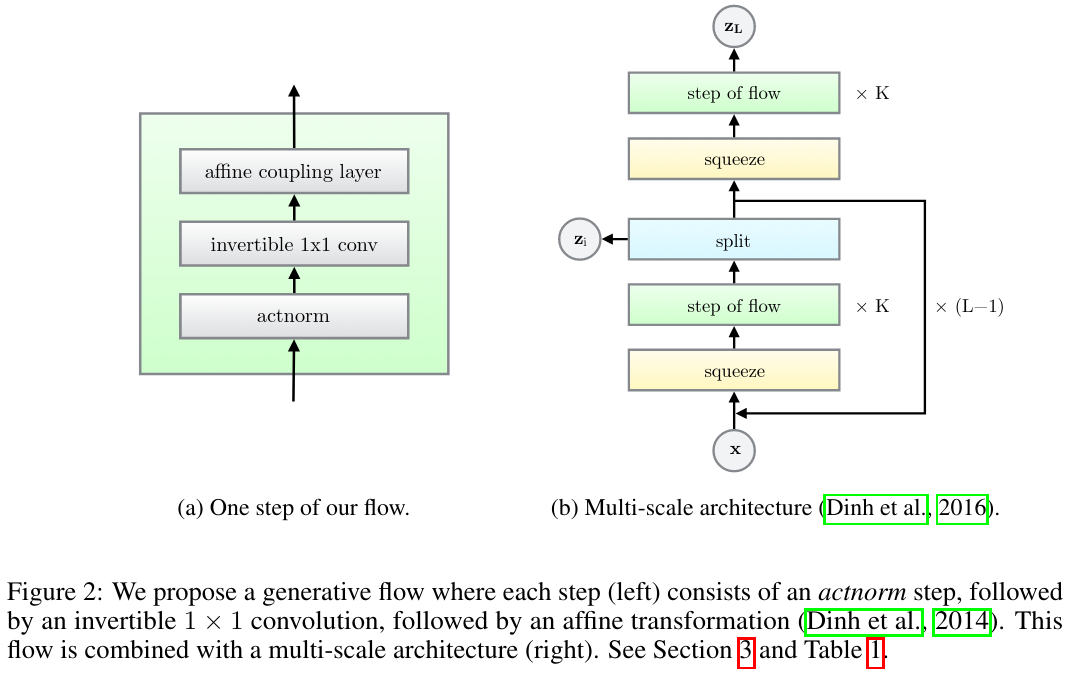
\includegraphics[width=\textwidth]{GLOWModel.png}
\end{frame}

\begin{frame}
    \frametitle{GLOW: What Changed?}
    \center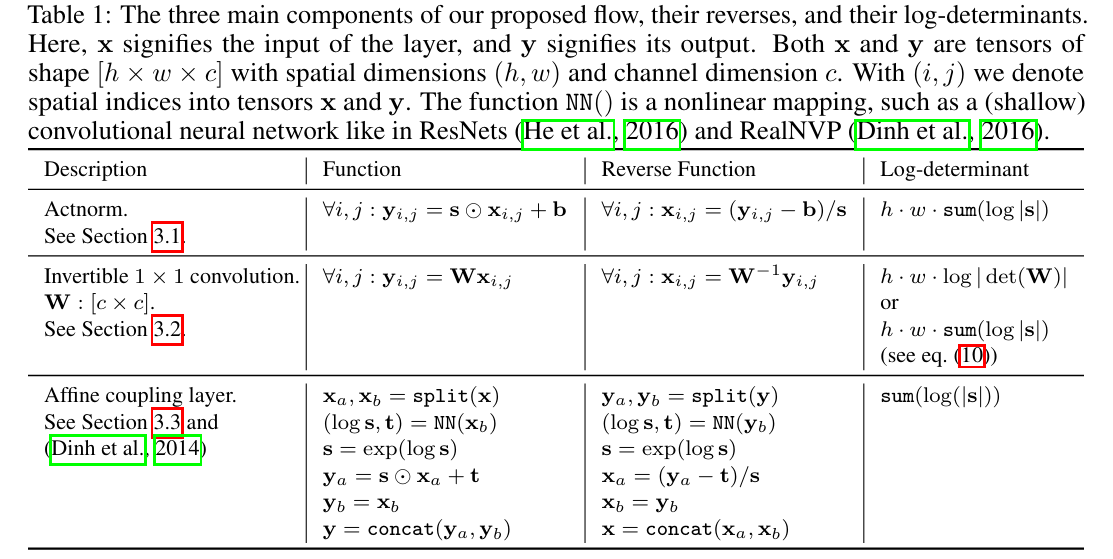
\includegraphics[width=\textwidth]{GLOWComponents.png}
\end{frame}

\begin{frame}
    \frametitle{GLOW: Training}
    \begin{itemize}
        \item Set $K=32$ and $L=6$ for ($32*6 + 32$) $224$ flow steps (NICE had
            5!)
        \item New type of layers (NICE only had the additive coupling)
        \item Can train on CelebA-HQ (256x256) images.
    \end{itemize}
\end{frame}

\begin{frame}
    \frametitle{GLOW: Results}
    \center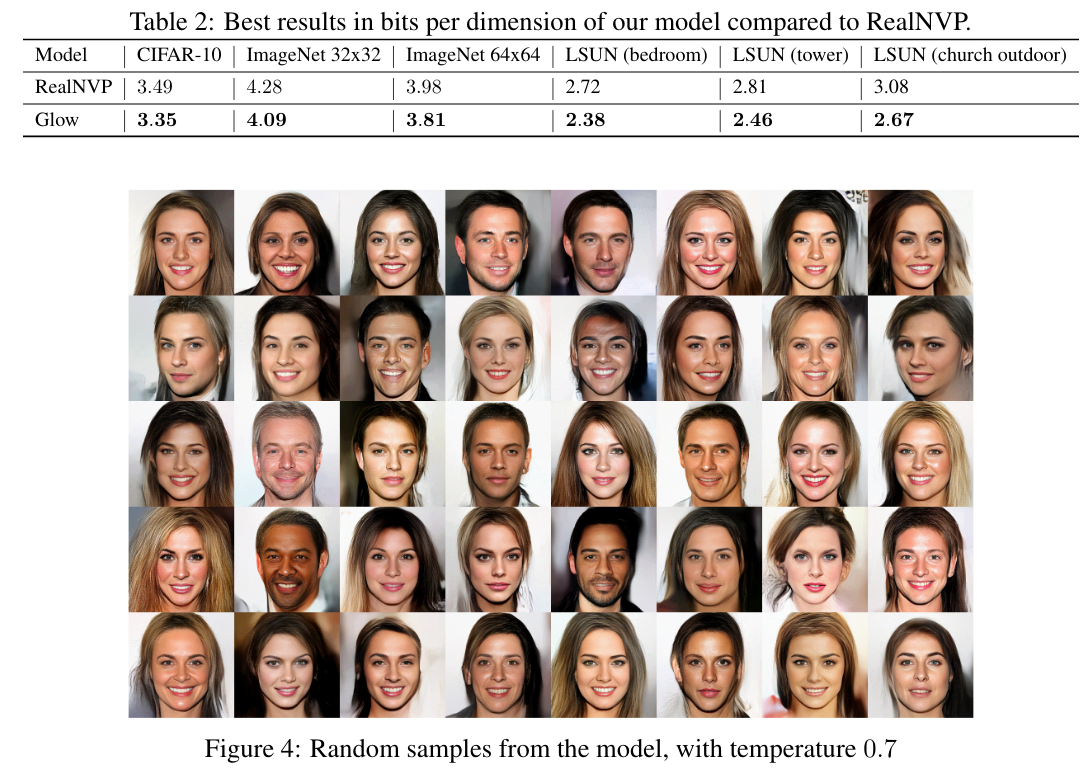
\includegraphics[width=\textwidth]{GLOWResults.png}
\end{frame}

\begin{frame}
    \frametitle{GLOW vs StyleGAN vs StyleGAN2}
    \begin{columns}
        \begin{column}{0.3\paperwidth}
            \center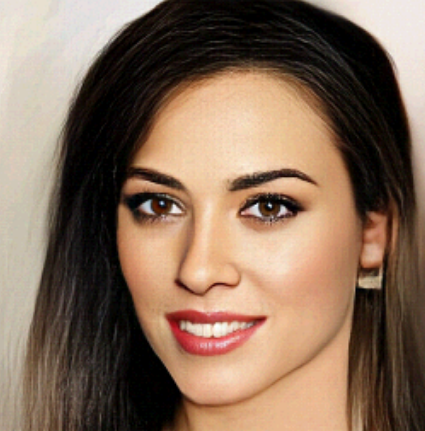
\includegraphics[width=\textwidth]{GLOWSingle.png}
            \\
            \center{GLOW}
        \end{column}
        \begin{column}{0.3\paperwidth}
            \center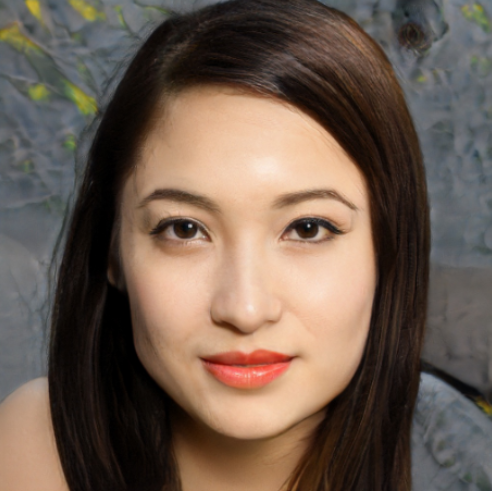
\includegraphics[width=\textwidth]{SRGAN.png}
            \\
            \center{StyleGAN}
        \end{column}
        \begin{column}{0.3\paperwidth}
            \center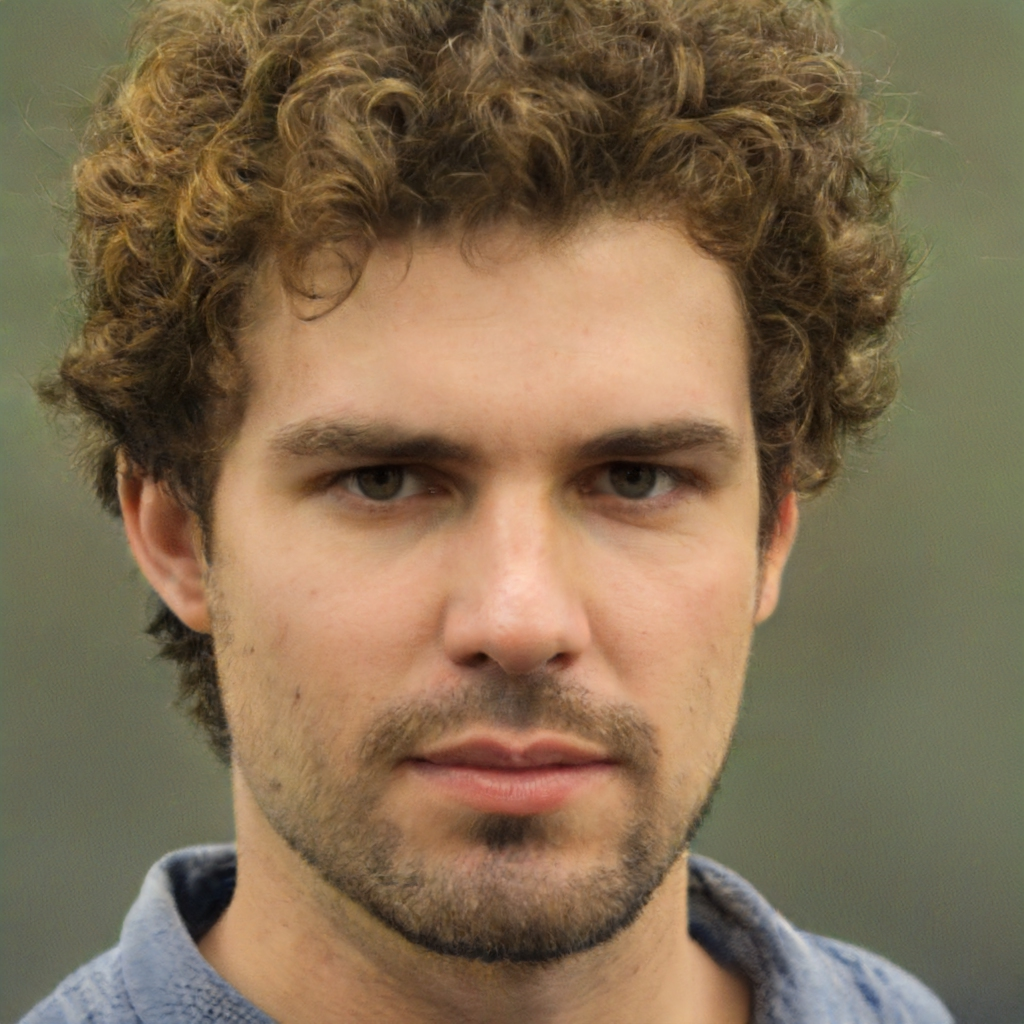
\includegraphics[width=\textwidth]{tpdne.jpg}
            \\
            \center{StyleGAN2}
        \end{column}
    \end{columns}
\end{frame}

\begin{frame}
    \frametitle{GLOW Downstream Tasks: Interpolation}
    \center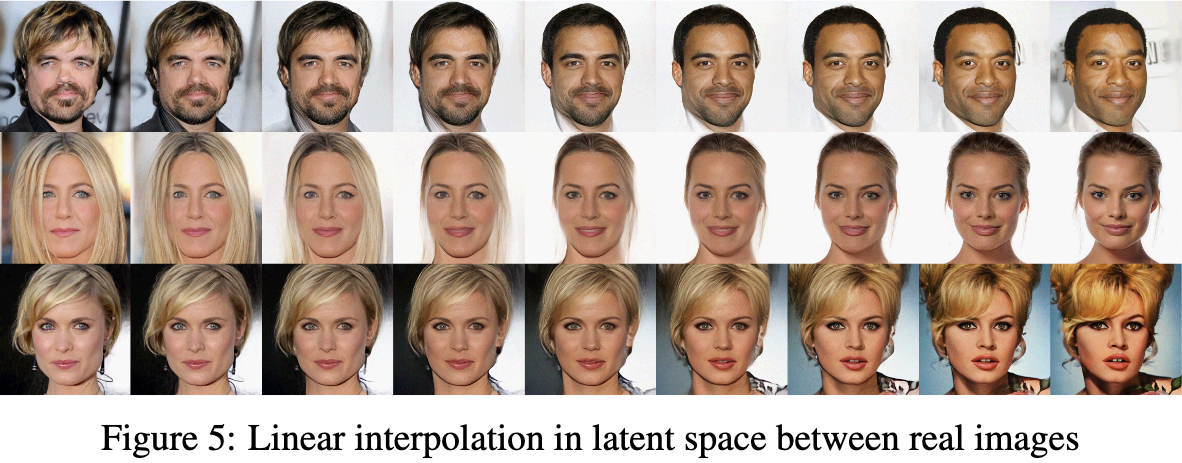
\includegraphics[width=\textwidth]{GLOWInterp.png}
\end{frame}

\begin{frame}
    \frametitle{GLOW Downstream Tasks: Feature Manipulation}
    \center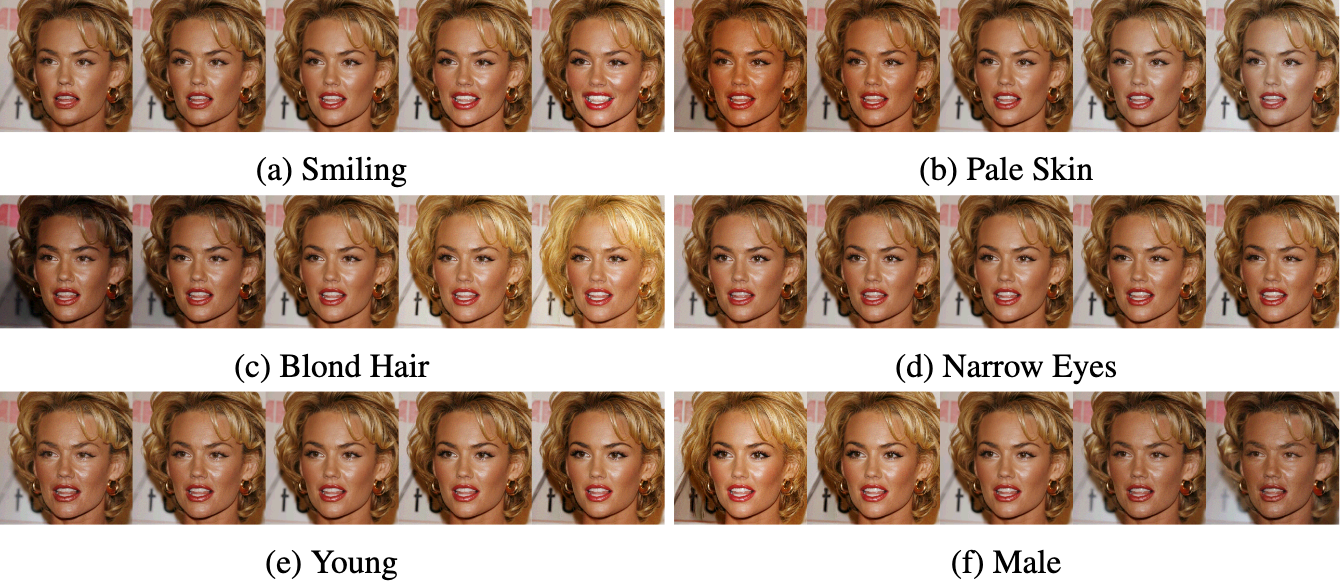
\includegraphics[width=\textwidth]{GLOWFeatures.png}
\end{frame}

\begin{frame}
    \frametitle{What About Using Flows for Super Resolution?}
    \begin{itemize}
        \item Use flows as a replacement for GAN super resolution.
        \item Training within certain scale uses a normalizing flow.
        \item When scaling up and down use injective and surjective functions.
        \item Output is a distribution instead of a single image.
    \end{itemize}
\end{frame}

\begin{frame}
    \frametitle{SRFlow}
    \center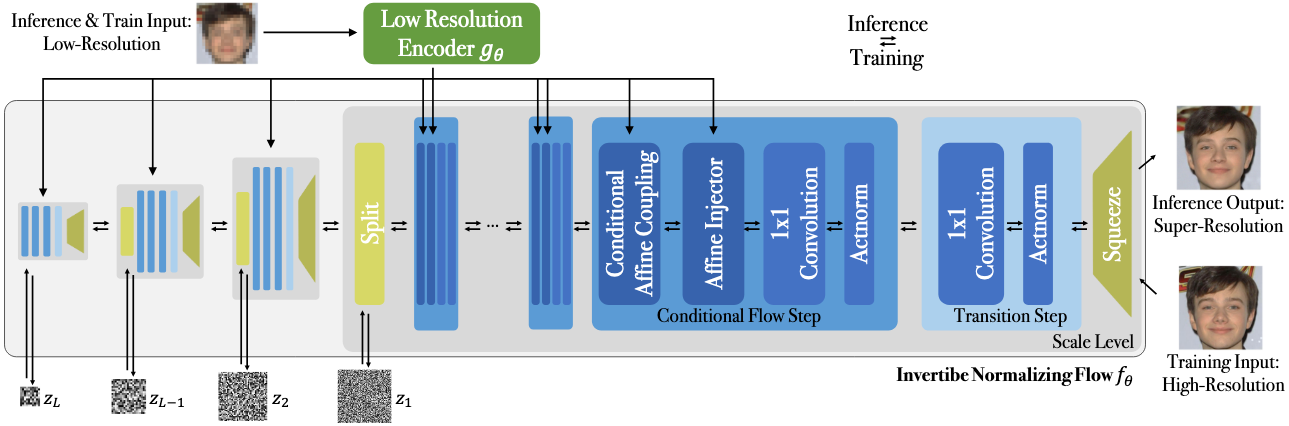
\includegraphics[width=\textwidth]{SRFLOW.png}
\end{frame}

\begin{frame}
    \frametitle{SRFlow: Comparison}
    \center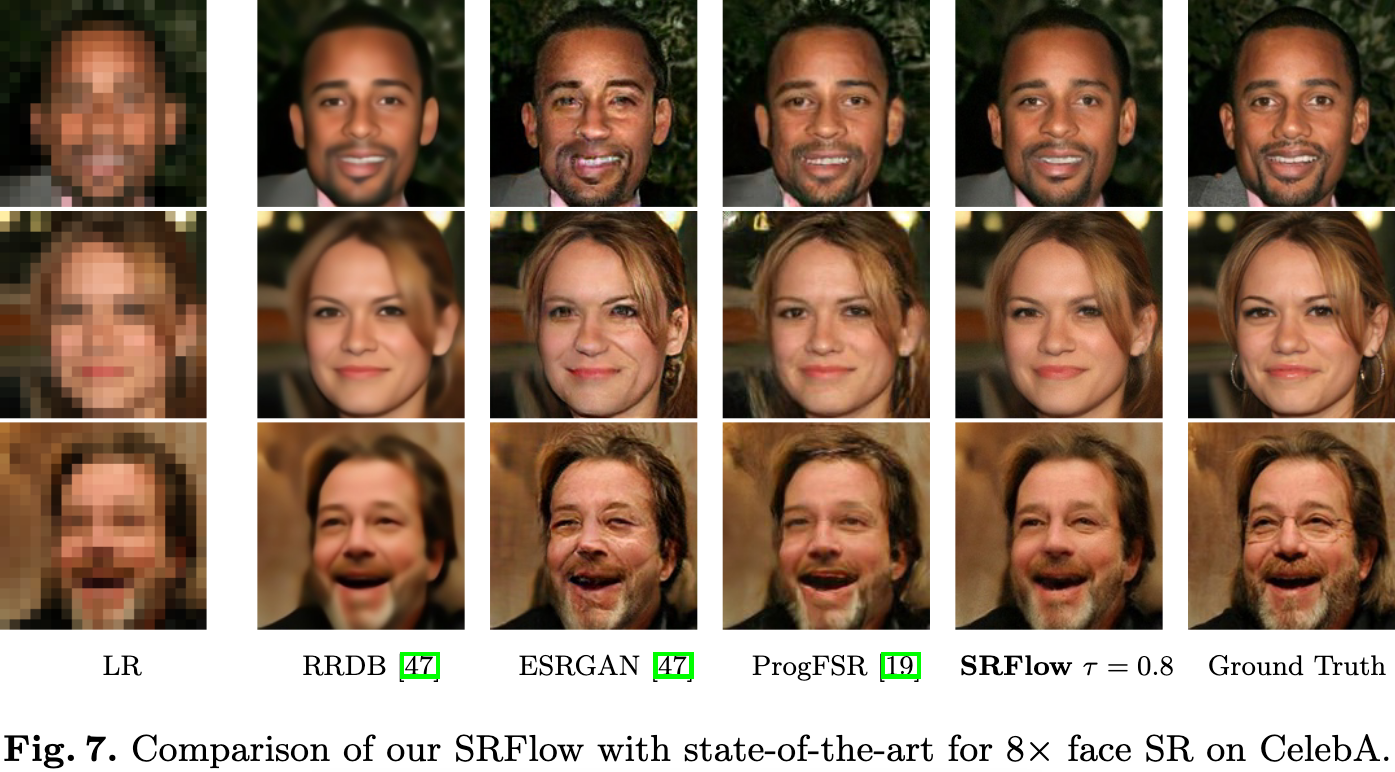
\includegraphics[width=\textwidth]{SRFLOW_Examples.png}
\end{frame}

\begin{frame}
    \frametitle{SRFlow: Stochastic Output}
    \center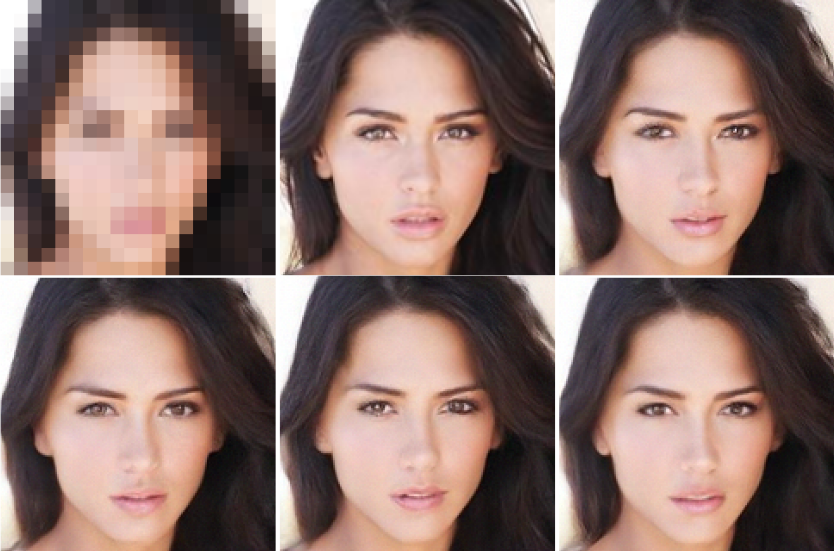
\includegraphics[width=\textwidth]{SRFLOW_Stochastic.png}
\end{frame}

\begin{frame}
    \frametitle{SRFlow: Stochastic Output}
    \center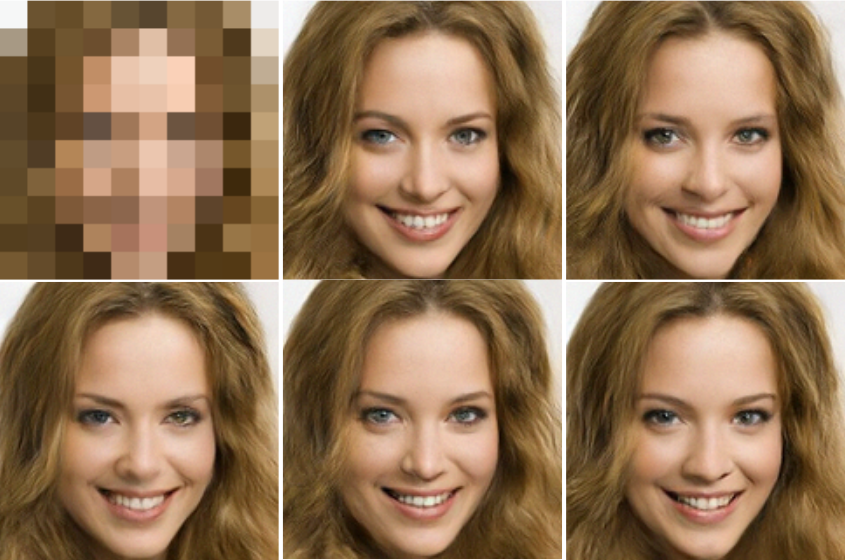
\includegraphics[width=\textwidth]{SRFLOW_Stochastic2.png}
\end{frame}


\begin{frame}
    \frametitle{Recap: Generative Models}
    \center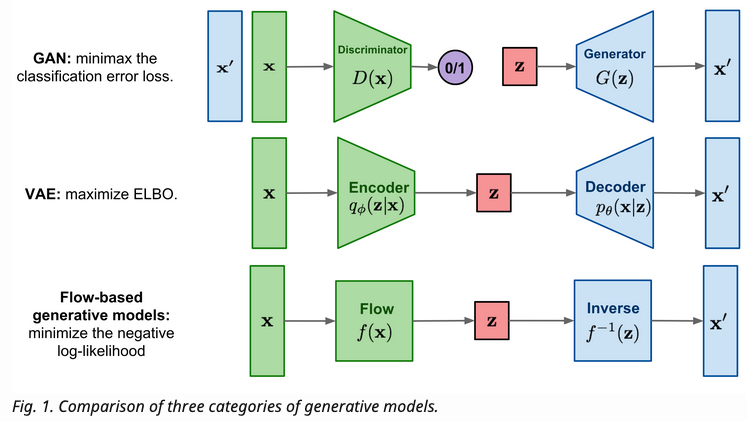
\includegraphics[width=\textwidth]{GenerativeModels.png}
\end{frame}

